\documentclass[11pt]{article}

\usepackage[review]{acl}

\usepackage{times}
\usepackage{latexsym}
\usepackage[T1]{fontenc}
\usepackage[utf8]{inputenc}
\usepackage{microtype}
\usepackage{inconsolata}
\usepackage{graphicx}
\usepackage{booktabs}
\usepackage{amsmath}
\usepackage{enumitem}
\usepackage[normalem]{ulem}
\usepackage{listings}

\setlength{\textfloatsep}{10pt plus 2pt minus 4pt}
\setlength{\floatsep}{10pt plus 2pt minus 4pt}
\setlength{\dbltextfloatsep}{10pt plus 2pt minus 4pt}
\setlength{\dblfloatsep}{10pt plus 2pt minus 4pt}

\title{How Does Schema Complexity Predict Performance\\in Training-Free LLM Information Extraction?}

\author{Anonymous}

\begin{document}
\maketitle

\begin{abstract}
Schema complexity affects training-free large language model (LLM) information extraction (IE), yet prior work conflates two factors: having more types to discriminate among (count) and having semantically similar types to confuse (confusability). We present, to our knowledge, the first controlled study isolating these factors in zero-shot LLM IE across four datasets, focusing on relation extraction (RE) as the primary testbed with named entity recognition (NER) and event detection as boundary conditions.
Using embedding-based confusability metrics with controlled batch design, we find:
(1)~count degradation spans NER and RE (up to $-$49 percentage points [pp]), and inter-type confusability independently predicts RE type substitution errors, with bounded interaction confirmed by equivalence testing;
(2)~batch confusability independently explains ${\sim}$27\% of cross-batch RE accuracy variance on FewRel (semipartial $R^2 = 0.273$), replicating across two model families at three scales (8B--70B), while the NER null serves as a boundary condition;
(3)~schema decomposition fails due to merge amplification and routing failure, though oracle routing recovers accuracy\footnote{Code and data are available at \url{https://anonymous.4open.science/r/schema-dag-extraction-4C10/}.}.
\end{abstract}


\section{Introduction}
\label{sec:introduction}

\begin{figure}[t]
\centering
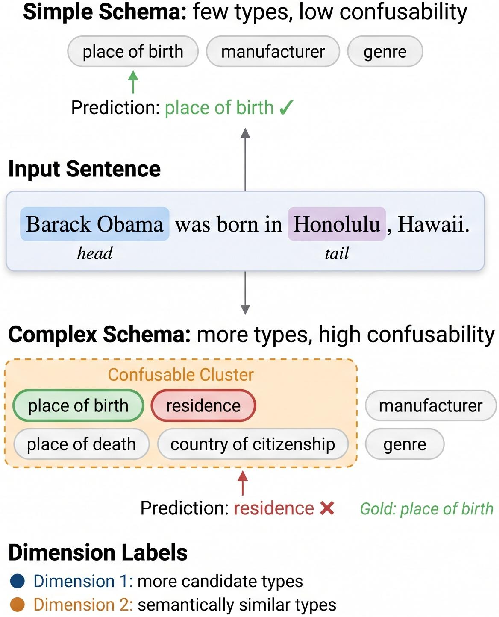
\includegraphics[width=\columnwidth]{../../figures/paper/fig_problem_illustration.pdf}
\caption{Schema complexity in zero-shot relation extraction. Given the same input, a simple schema (few dissimilar types) yields the correct relation, while a complex schema with more candidate types and a cluster of semantically similar types causes type substitution (gold \emph{place of birth} $\to$ predicted \emph{residence}). We decompose schema complexity into two dimensions: type count and inter-type confusability.}
\label{fig:problem}
\end{figure}

\looseness=-1
Training-free\footnote{We use ``training-free'' and ``zero-shot'' interchangeably to denote prompting without parameter updates.} LLM information extraction (prompting a large language model with a target schema and asking it to extract structured information without any task-specific fine-tuning) enables rapid deployment across new domains and ontologies. This zero-shot paradigm eliminates the need for labeled data, and is attractive for applications where annotation is expensive or schemas evolve frequently \citep{llm4ie-survey-2024}. Yet the paradigm carries a critical limitation: performance degrades sharply as the number of candidate types in the prompt schema grows. On named entity recognition, recall drops from 0.72 with a single candidate type to a plateau of ${\sim}$0.28 across intermediate schema sizes (22--44 types) before partial recovery at full-schema. On relation extraction, accuracy falls from 85.7\% with one relation to 50.4\% with 80 relations (sentence-level) and from 88.0\% to 38.7\% with 96 relations (document-level), near-halving or worse. This degradation is not academic: real-world ontologies routinely define 50--200+ types, which places them squarely in the regime where training-free extraction becomes unreliable (Figure~\ref{fig:problem}).

\looseness=-1
What explains this degradation? Prior decomposition strategies \citep{uniner-2024,llm-pee-2025,parse-2025} conflate two factors: having more types to discriminate among (count) and having semantically similar types to confuse (confusability) (hereafter Dimension~1 and Dimension~2). None isolates which factor predicts the gains (\S\ref{sec:related_work}).

This study combines correlational analyses with quasi-experimental manipulation (confusability-controlled batches) to characterize how schema properties predict extraction accuracy (Figure~\ref{fig:framework}).

We ask three questions. \textbf{RQ1}: Does type confusability independently predict extraction degradation beyond the effect of type count? \textbf{RQ2}: Through what modes do count and confusability each degrade performance? \textbf{RQ3}: Can confusability-aware schema decomposition improve extraction quality?

\looseness=-1
To our knowledge, we present the first controlled study simultaneously isolating type count and inter-type confusability as independent dimensions via embedding-based metrics and stratified batch design in zero-shot LLM IE, spanning NER, RE, and event detection (ED). We quantify confusability using pairwise embedding similarity, the \emph{Schema Confusability Score} (SCS), and its batch-level aggregation, the \emph{Batch Confusability Score} (BCS). We evaluate on Few-NERD \citep{fewnerd-2021}, FewRel \citep{fewrel-2018}, DocRED \citep{docred-2019}, and MAVEN \citep{maven-2020} using Qwen3-32B (\S\ref{sec:experimental_setup}).

Our contributions are:
\begin{enumerate}[leftmargin=*,itemsep=2pt,topsep=2pt]
    \item We find that type confusability, quantified by embedding similarity (SCS/BCS, building on \citealt{llm-pee-2025}), independently predicts type substitution errors in RE on FewRel (variance inflation factor [VIF]${}\,=\,1.18$), independently explaining ${\sim}$27\% of batch-level variance (semipartial $R^2 = 0.273$; ecological level). This finding is enabled by BCS-controlled batch design that isolates confusability from type count, a methodology not previously applied in training-free LLM IE (\S\ref{sec:count_curves}, \S\ref{sec:pairwise}, \S\ref{sec:bcs_controlled}).
    \item We document a task-dependent boundary: the RE confusability effect is replicated across two model families (three scales), with no detected format dependence, while the NER batch-level BCS null (reported as a boundary condition rather than a negative result) is attributable to dispersed error modes (miss, boundary, type) and BCS range compression (\S\ref{sec:bcs_controlled}, \S\ref{sec:multi_channel}).
    \item We identify structural barriers to confusability-aware extraction: schema decomposition fails due to merge amplification (NER, ED) and routing failure (RE). The decompose-then-merge paradigm faces structural precision--recall tradeoffs in training-free IE (\S\ref{sec:sdgd}).
\end{enumerate}

% Figure 2 (fig:framework) moved to related_work.tex for page distribution

\section{Related Work}
\label{sec:related_work}

\paragraph{Training-free LLM IE.}
\looseness=-1
Training-free LLM IE spans instruction tuning \citep{instructuie-2023}, code-style schema encoding \citep{knowcoder-2024,codeie-2023}, annotation-guided extraction \citep{gollie-2024,adelie-2024}, schema-driven decoding \citep{slot-2025,oneke-2025}, and constrained JSON decoding \citep{json-schema-bench-2025,willard2023efficient}. NER methods include zero-shot decomposition \citep{xie-zeroshot-ner-2023,promptner-2023}, distillation \citep{uniner-2024}, and bidirectional encoders \citep{gliner-2024,gliner2-2025}; RE methods include zero-shot triplet extraction \citep{relationprompt-2022}, constrained generation \citep{josifoski-2022-genie}, and shared embedding spaces \citep{boylan-2025-glirel,wadhwa-re-llm-2023}. Related work exploits type embeddings for retrieval \citep{shachar-2025-ner-retriever} and introspective confusion for example selection \citep{reflect-learn-2026}. These methods handle moderate schemas (4--20 types) but none investigates how performance degrades as schema complexity scales.

\begin{figure}[t]
\centering
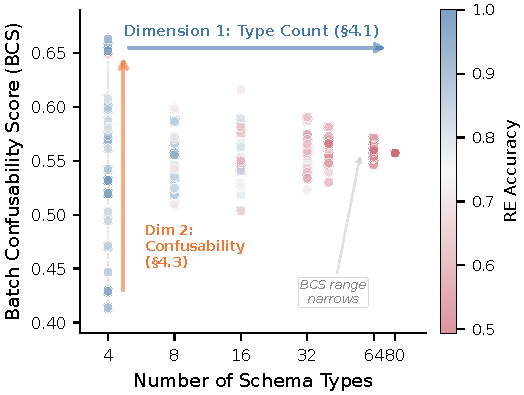
\includegraphics[width=\columnwidth]{../../figures/paper/fig_framework.pdf}
\caption{Experimental design overview on FewRel. Each point is one batch; color encodes RE accuracy (green=high, red=low). \textbf{Dimension~1} (horizontal): accuracy declines with type count (\S\ref{sec:count_curves}). \textbf{Dimension~2} (vertical): within each count level, higher BCS correlates with lower accuracy (\S\ref{sec:bcs_controlled}). BCS range narrows at high counts, limiting Dimension~2 discriminability.}
\label{fig:framework}
\end{figure}

\paragraph{Schema complexity in IE.}
\looseness=-1
The most directly related work is LLM-PEE \citep{llm-pee-2025}, which partitions large event schemas by type embedding similarity. Our work differs in three ways: (1)~we conduct controlled analysis to understand \emph{why} extraction degrades rather than developing an engineering solution; (2)~our BCS-controlled experiments isolate count from confusability with verified orthogonality ($\text{VIF}=1.18$), which LLM-PEE conflates without controlling for confounding variables; (3)~our decomposition experiments (\S\ref{sec:sdgd}) reveal that merge amplification (not partitioning quality) is the bottleneck in decompose-then-merge pipelines. LLM-PEE's union merge suffers the same precision collapse (0.56$\to$0.21; \S\ref{sec:sdgd}). In short, LLM-PEE assumes decomposition helps; we show why it should (confusability), why it does not (merge amplification), and what predicts the degradation (BCS). Other approaches address schema complexity via hard negative mining \citep{iepile-2024}, schema definition optimization \citep{parse-2025}, multi-agent debate \citep{crossagentie-2025,cmas-ner-2025}, and active prompting \citep{reflect-learn-2026}; all treat it as an engineering problem rather than isolating degradation factors. Concurrently, \citet{chen-2026-multi-instance} show that instance count degrades LLM multi-instance processing more than context length, consistent with our count-dominant finding. \citet{golde-2025-familiarity} quantify training--evaluation type similarity to predict zero-shot NER difficulty; our SCS instead measures within-schema inter-type confusability without assuming access to training data. Label-space reduction approaches \citep{haystack-to-needle-2025,dlisc-2025,spt-2025} implicitly lower batch confusability; our framework explains \emph{why} such reduction works.

\paragraph{Schema complexity beyond IE.}
\looseness=-1
Schema-dialogue benchmarks \citep{rastogi2020towards,lee2022sgd} and \citet{li2023evaluating} document count-dependent LLM IE degradation. The link between label similarity and confusion has precedent in vision \citep{dubey-2018-pairwise-confusion,deng-2010-imagenet} and label noise \citep{collier-2021-correlated-noise,guo-2021-label-confusion}.

\paragraph{SCS novelty.}
\looseness=-1
SCS inherits the embedding-similarity criterion from LLM-PEE \citep{llm-pee-2025}, repurposed from schema partitioning to controlled analysis; parallels exist in metric learning \citep{snell2017prototypical} and zero-shot classification \citep{yin-2019-zero-shot-bench}. The modest pairwise $r^2$ (1.3--1.7\%) compounds at the batch level to explain substantial cross-batch RE variance (\S\ref{sec:bcs_controlled}).

\begin{table}[t]
\centering
\small
\resizebox{\columnwidth}{!}{%
\begin{tabular}{llrrlll}
\toprule
\textbf{Dataset} & \textbf{Task} & \textbf{\# Types} & \textbf{\# Eval Units} & \textbf{Domain} & \textbf{BCS Range} & \textbf{Embedding} \\
\midrule
Few-NERD & NER & 66 & 1{,}000 & Cross & 0.77--0.93 & Qwen3-32B \\
FewRel & RE (sent.) & 80 & 1{,}000 & Cross & 0.42--0.97 & MiniLM \\
DocRED & RE (doc.) & 96 & 1{,}000 & Cross & 0.53--0.73 & MiniLM \\
MAVEN & ED & 168 & 18{,}904\rlap{$^\dagger$} & Same & 0.87--0.97 & MiniLM \\
\bottomrule
\end{tabular}}
\caption{Dataset statistics. BCS Range: min--max over count-curve batches. Embedding: model used for SCS/BCS; ranges are not comparable across embedding models. $^\dagger$Trigger mentions across 8{,}042 sentences.}
\label{tab:datasets}
\end{table}



\section{Experimental Setup}
\label{sec:experimental_setup}

\looseness=-1
We evaluate how prompt schema size and inter-type confusability affect zero-shot LLM extraction across three information extraction tasks and four datasets: named entity recognition (NER), sentence-level relation extraction (RE), document-level RE, and event detection (ED).

\begin{figure*}[t]
\centering
\begin{minipage}[t]{0.48\textwidth}
\centering
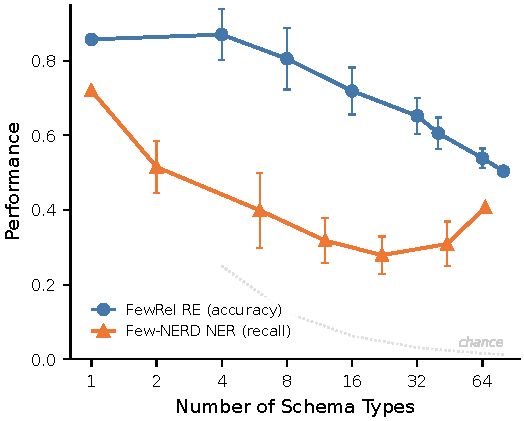
\includegraphics[width=\linewidth]{../../figures/paper/fig_count_curves.pdf}
\end{minipage}
\hfill
\begin{minipage}[t]{0.48\textwidth}
\centering
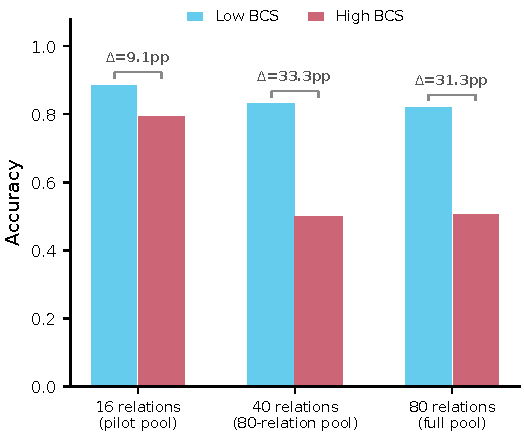
\includegraphics[width=\linewidth]{../../figures/paper/fig_bcs_scaling.pdf}
\end{minipage}
\caption{\textbf{(a)} Count-degradation curves. Error bars: $\pm 1$ standard deviation (SD) across 3 batch-composition seeds $\times$ 25 batches. RE declines monotonically; NER shows a U-shape. Rightmost points are full-schema (negligible sampling variance). \textbf{(b)} Illustrative BCS-controlled FewRel accuracy: each bar represents one extreme-BCS batch per condition. Slopes are consistent across pool conditions ($p = 0.60$); wider BCS range at 80 relations produces larger gaps. Statistical evidence is provided by the pooled regression (\S\ref{sec:bcs_controlled}, semipartial $R^2 = 0.273$, $n = 204$).}
\label{fig:main_results}
\end{figure*}

\subsection{Tasks and Datasets}
\label{sec:datasets}

\paragraph{Few-NERD (NER).}
\looseness=-1
Few-NERD \citep{fewnerd-2021} provides 66 fine-grained entity types organized into 8 coarse categories (person, location, organization, building, art, product, event, other). The dataset spans diverse domains. We sample 1{,}000 instances uniformly from the test set; type frequency follows the natural long-tail distribution of Few-NERD. Evaluation uses token-level text matching. Pairwise analysis covers 1{,}953 type pairs with non-zero co-occurrence out of $\binom{66}{2}=2{,}145$ possible pairs.

\paragraph{FewRel (RE).}
\looseness=-1
FewRel \citep{fewrel-2018} contains 80 relation types sourced from Wikidata. Since the validation split covers only 16 relations, we combine the training and validation splits to obtain the full 80-relation pool required for schema-scale experiments. We sample 1{,}000 balanced instances (12--13 per relation type, stratified to ensure equal representation). A held-out validation confirms SCS--confusion generalization across the split boundary (Appendix~\ref{app:scs-heldout-validation}). Each instance provides a sentence with marked head and tail entities; the task is to classify the relation. FewRel's balanced design (700 instances per relation type) eliminates type frequency as a potential confound; this balance makes it the primary dataset for BCS analysis. Contamination analysis (Appendix~\ref{app:split-origin}) shows extraction difficulty correlates inversely with training-set prevalence, and BCS effects are unchanged when controlling for contamination.

\paragraph{DocRED (Document-level RE).}
\looseness=-1
DocRED \citep{docred-2019} contains 96 relation types sourced from Wikidata, evaluated at the document level where entity pairs may span multiple sentences. We sample 1{,}000 instances balanced across 96 relation types ($\sim$10 per type) from the DocRED development set. The task is formulated identically to FewRel: given a document with marked head and tail entities, classify the relation. We use the development set, as DocRED test labels require submission to a hidden evaluation server. DocRED extends the RE evaluation to a larger schema (96 vs.\ 80 types) and document-level context, testing whether confusability effects persist under longer input contexts and cross-sentence reasoning.

\paragraph{MAVEN (ED).}
MAVEN \citep{maven-2020} defines 168 event types derived from the FrameNet ontology; all types belong to a single ontology (FrameNet), so this is a same-domain schema. We use the validation set (8{,}042 sentences containing 18{,}904 event mentions) for evaluation, as test set labels are not publicly available. The task requires both trigger identification and event type classification. MAVEN serves a supplementary role: its same-domain schema produces centrality confounds at the batch level (\S\ref{sec:centrality_confound}), and its compressed BCS range (0.87--0.97) limits the variance available for regression analysis.

Table~\ref{tab:datasets} summarizes the dataset statistics, including the Schema Confusability Score (SCS) ranges defined in \S\ref{sec:scs}.

% Table 1 (tab:datasets) moved to end of related_work.tex for page-3 placement

\subsection{Schema Confusability Score (SCS)}
\label{sec:scs}

\looseness=-1
We define the Schema Confusability Score (SCS) to quantify semantic overlap between types in a schema. Given a type $t$ with name string $\text{name}(t)$, an embedding function $\text{embed}(\cdot)$ maps the type name to a vector representation. The \textbf{pairwise SCS} between types $t_i$ and $t_j$ is:
{\small
\[
\text{SCS}(t_i, t_j) = \cos\bigl(\text{embed}(\text{name}(t_i)),\; \text{embed}(\text{name}(t_j))\bigr)
\]
}

We use mean pairwise SCS as the default BCS aggregation; max-based BCS yields directionally consistent results (Appendix~\ref{sec:appendix_bcs_sensitivity}, Table~\ref{tab:bcs_aggregation}). BCS captures confusability-specific signal beyond type composition (Appendix~\ref{app:bcs-composition}).

For a batch of types $B = \{t_1, \ldots, t_k\}$, the \textbf{Batch Confusability Score (BCS)} aggregates all pairwise similarities:
\[
\text{BCS}(B) = \frac{1}{\binom{k}{2}} \sum_{i < j,\; t_i, t_j \in B} \text{SCS}(t_i, t_j)
\]

\looseness=-1
We compute SCS with two embeddings: (1)~Qwen3-32B \citep{qwen3-2025} hidden-state representations (5{,}120-d) and (2)~all-MiniLM-L6-v2 \citep{minilm-2020,sentence-bert-2019}, a 384-d sentence encoder. MiniLM is the primary BCS embedding; cross-embedding consistency holds on all datasets, with MiniLM yielding equal or stronger correlations (Appendix~\ref{sec:appendix_bcs_sensitivity}). Few-NERD uses Qwen3 because its fine-grained same-category pairs require the higher-dimensional space. Name-only SCS yields equivalent predictive accuracy to name+definition (Appendix~\ref{app:scs-ablation}).

\paragraph{SCS as a lightweight proxy.}
\label{sec:scs-validation}
SCS is a pre-hoc proxy computable without running extraction; pairwise correlations with observed type confusion are reported in \S\ref{sec:pairwise}. SCS does not capture context-dependent disambiguation or mention-level ambiguity; these contribute to residual variance.

\begin{figure}[t]
\centering
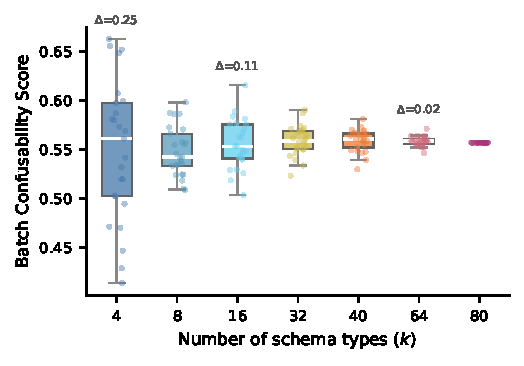
\includegraphics[width=\columnwidth]{../../figures/paper/fig_bcs_scatter.pdf}
\caption{BCS range compression on FewRel: as type count $k$ increases, achievable BCS range narrows ($\Delta{=}0.25$ at $k{=}4$ to $\Delta{<}0.01$ at $k{=}80$), limiting power to detect confusability effects without extreme-BCS construction (\S\ref{sec:exp_design}). Each point is one of 25 random batches; boxes show IQR.}
\label{fig:bcs_range}
\end{figure}

\subsection{Experimental Design}
\label{sec:exp_design}

We conduct two complementary experiments.

\paragraph{Experiment 1: Count Curves.}
\looseness=-1
We vary the number of types presented in the prompt schema to measure performance as a function of schema size. For each count level, we sample 25 random type batches for Few-NERD and FewRel (5 for DocRED and MAVEN)\footnote{DocRED and MAVEN use fewer batches due to higher per-batch evaluation cost (document-level RE and 8{,}042 sentences, respectively).} and evaluate against the same 1{,}000-sample pool. For NER and ED, all samples are evaluated in every batch; for RE, each batch evaluates only the subset whose gold relation appears in the candidate set ($k/K$ of the pool, where $K$ is the total number of types), so effective sample size scales with count. At count${}=1$, every type is evaluated individually as a solo baseline. The remaining count levels follow natural partition points in each schema's type hierarchy rather than uniform spacing: \{2, 6, 12, 22, 44, 66\} for Few-NERD, \{4, 8, 16, 32, 40, 64, 80\} for FewRel, \{4, 8, 16, 32, 64, 96\} for DocRED, and \{6, 12, 22, 44, 64\} for MAVEN.

\paragraph{Experiment 2: BCS-Controlled.}
\looseness=-1
We fix type count and vary BCS to isolate confusability from schema size. For each count level, we construct one low-BCS batch, one high-BCS batch, and 25 random batches (27 total). We construct extreme batches via greedy search over the pairwise SCS matrix. The low-BCS batch starts from the least-similar type pair and iteratively adds the type with lowest maximum similarity to already-selected types; the high-BCS batch mirrors this with maximum similarity. This design is motivated by BCS range compression: random batches exhibit narrowing BCS variance at higher counts ($\Delta = 0.25$ at $k{=}4$ vs.\ $< 0.01$ at $k{=}80$; Figure~\ref{fig:bcs_range}), limiting statistical power to detect confusability effects without extreme-BCS construction. We evaluate on Few-NERD (count$\,\in\{6, 12\}$), FewRel (count$\,\in\{8, 16\}$, both 16-relation (pilot) and 80-relation pools), and DocRED (count$\,\in\{16, 32\}$). Within-pool 16-relation subsets from the 80-relation pool isolate confusability from pool composition. MAVEN results are reported separately due to a centrality confound (\S\ref{sec:centrality_confound}).

\subsection{Evaluation Metrics}
\label{sec:metrics}

\textbf{NER}: text-match F1 (exact string + type match). \textbf{RE}: accuracy (exact relation label match; each batch evaluates only samples whose gold relation is among the candidates; \texttt{none} responses scored as incorrect). \textbf{ED}: relaxed F1 (token overlap + correct event type).


\subsection{Model and Inference}
\label{sec:model}

\looseness=-1
We use Qwen3-32B-FP8 \citep{qwen3-2025} served via vLLM v0.20.2 \citep{vllm-2023} on a single NVIDIA RTX PRO 6000 GPU (96\,GB) with greedy decoding (temperature${}\,=\,0$, seed 42). Two NER/ED prompt versions are evaluated: v1 requests character offsets; v2 adds format constraints that double precision with minimal recall loss. RE uses a single prompt version throughout (templates and type definitions in Appendix~\ref{sec:appendix_prompts}). The BCS--accuracy relationship is format-independent: constrained and unconstrained decoding yield identical correlations (Appendix~\ref{app:format-independence}). Cross-model validation uses Meta-Llama-3.1-70B-Instruct (FP8) and Meta-Llama-3.1-8B-Instruct \citep{llama3-2024}. Single-seed greedy decoding substantially reduces model-level randomness (residual SD${}\,=\,0.88$\,pp; Appendix~\ref{app:variance-decomposition}); bootstrap CIs capture batch-composition variance ($B{=}10{,}000$ pairwise; $B{=}1{,}000$ batch-level). Total computation is ${\sim}$72 GPU-hours on a single RTX PRO 6000.


\section{Results}
\label{sec:results}

All experiments use Qwen3-32B and the v1 prompt (\S\ref{sec:model}; Appendix~\ref{sec:appendix_prompts}) unless noted; cross-model validation covers Dimensions~1--2, while secondary analyses (error taxonomy, DocRED $R^2$, Two One-Sided Tests [TOST]) remain single-model.

\begin{table}[t]
\centering
\small
\resizebox{\columnwidth}{!}{%
\begin{tabular}{llrrrrr}
\toprule
\textbf{Dataset} & \textbf{Embed.} & \textbf{$n$ pairs} & \textbf{$r$} & \textbf{$r^2$} & \textbf{95\% CI} & \textbf{$p$} \\
\midrule
Few-NERD & Qwen3 & 1{,}953 & 0.112 & 0.013 & {[}0.076, 0.156{]} & ${<}\,0.001$ \\
MAVEN & MiniLM & 11{,}026 & 0.129 & 0.017 & {[}0.104, 0.156{]} & ${<}\,0.001$ \\
\bottomrule
\end{tabular}}
\caption{Pairwise SCS--confusion correlation. Confusion rate is bidirectional $C(t_i{\to}t_j) + C(t_j{\to}t_i)$ divided by gold frequency sum; CIs are percentile bootstrap ($B{=}10{,}000$). FewRel ($r = 0.187$; \S\ref{sec:scs-validation}) excluded (per-instance RE format). Type-level cluster bootstrap CIs exclude zero (Few-NERD [0.069, 0.219]; MAVEN [0.081, 0.185]).}
\label{tab:pairwise}
\end{table}

\subsection{Count-Degradation Curves}
\label{sec:count_curves}

\looseness=-1
Figure~\ref{fig:main_results}a shows RE accuracy declines monotonically with schema size (85.7\%$\to$50.4\% for FewRel). NER recall drops from 0.72 (count 1) to 0.28 before recovering to 0.41 at full-schema. DocRED replicates the monotonic RE pattern (88.0\%$\to$38.7\%; Appendix~\ref{sec:appendix_figures}); MAVEN exhibits a reversed trend attributable to centrality confounding (\S\ref{sec:centrality_confound}). The decline is stable across seeds (Jonckheere-Terpstra $p < 0.001$) and replicates on Llama-8B ($-$43\,pp; Table~\ref{tab:cross_model}), Llama-70B, and Gemini Flash (Figure~\ref{fig:cross_model_count}).

\subsection{Pairwise Confusability and Type Confusion}
\label{sec:pairwise}

\looseness=-1
We test whether pairwise SCS predicts type-level confusion rates. For each type pair $(t_i, t_j)$, we compute the confusion rate (the fraction of $t_i$ gold instances misclassified as $t_j$) and correlate it with $\text{SCS}(t_i, t_j)$. Table~\ref{tab:pairwise} reports Pearson correlations with bootstrap 95\% confidence intervals (CIs).

\looseness=-1
The correlations are statistically significant but modest: $r^2 \approx 1.3\text{--}1.7\%$. Type-level cluster bootstrap yields wider but still significant CIs (Few-NERD: [0.069, 0.219]; MAVEN: [0.081, 0.185]; $B = 10{,}000$). Spearman correlations corroborate ($\rho = 0.144\text{--}0.227$; reaching $0.27\text{--}0.31$ among nonzero-confusion pairs).

\looseness=-1
While pairwise $r^2$ is modest, correlated type pairs within batches compound into substantial batch-level RE accuracy variance (\S\ref{sec:bcs_controlled}). Independent MiniLM embeddings yield stronger correlations ($r = 0.172$ vs.\ Qwen3 $r = 0.138$; Appendix~\ref{sec:appendix_bcs_sensitivity}); SCS outperforms simpler baselines (Appendix~\ref{app:scs-baselines}; concrete examples in Appendix~\ref{app:error-analysis}).

\begin{figure}[t]
\centering
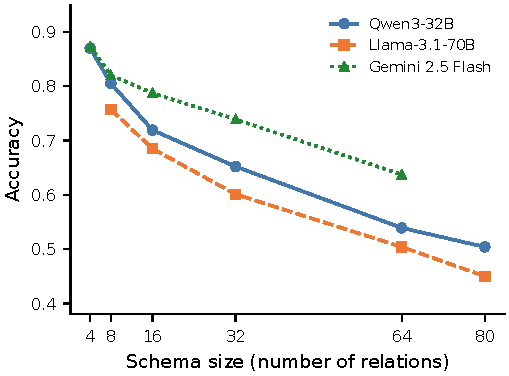
\includegraphics[width=\columnwidth]{../../figures/paper/fig_cross_model_count.pdf}
\caption{Cross-model count-curve replication on FewRel RE. All three model families show monotonic accuracy decline with schema size ($\rho = -1.0$ for Qwen3-32B and Gemini Flash on counts 4--32). Gemini shows shallower decline, consistent with ceiling compression.}
\label{fig:cross_model_count}
\end{figure}

\begin{figure*}[t]
\centering
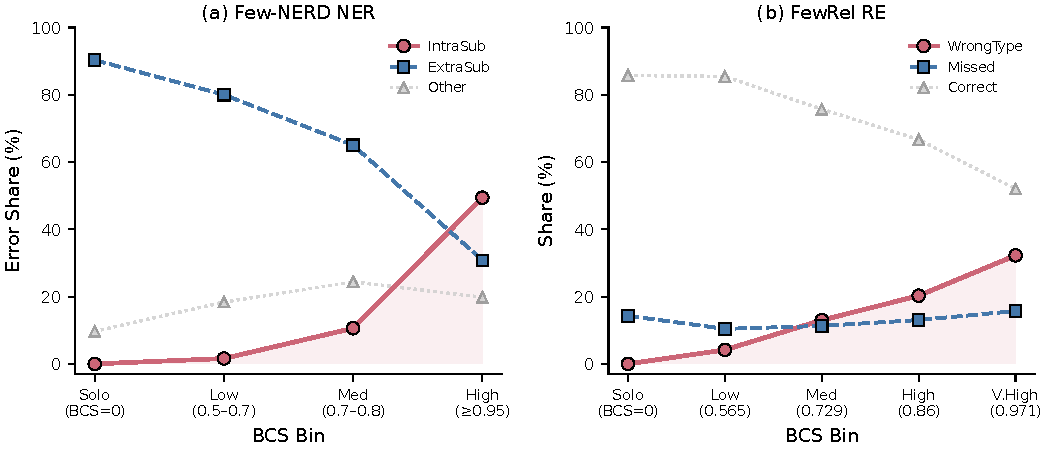
\includegraphics[width=\textwidth]{../../figures/paper/fig_error_taxonomy.pdf}
\caption{Error taxonomy decomposition (Few-NERD NER and FewRel RE). Intra-batch substitution (IntraSub) scales monotonically with BCS across all evaluated datasets ($\rho = 0.843\text{--}1.0$; Table~\ref{tab:error_taxonomy} includes DocRED). RE missed rates remain flat (10--16\%), but NER missed rates are substantially higher (43--65\%) and non-monotonic.}
\label{fig:error_taxonomy}
\end{figure*}

\subsection{BCS-Controlled Experiments}
\label{sec:bcs_controlled}

\looseness=-1
On FewRel, BCS independently explains ${\sim}$27\% of cross-batch RE accuracy variance (semipartial $R^2 = 0.273$, $n = 204$, after controlling for degree centrality), the primary quantitative evidence for confusability as a predictor alongside count. We fix type count and vary BCS to isolate this effect. FewRel's balanced design (700 instances per type) eliminates type frequency as a confound;\footnote{Partial correlation controlling for degree centrality: FewRel $r_{\text{partial}} = -0.537$ ($p < 0.001$, VIF${}\,=\,1.18$). DocRED partial correlation ($r_{\text{partial}} = -0.348$, $p < 0.001$) is reported for completeness, but VIF${}\,=\,50.9$ (BCS--centrality $r = 0.99$) renders the estimate unstable; the clean evidence for BCS's independent contribution comes from FewRel (Appendix~\ref{sec:appendix_partial_corr}, Table~\ref{tab:partial_corr}).} the within-pool analysis (\S\ref{sec:within_pool}) controls for pool composition. Adding domain entropy as a covariate leaves the BCS coefficient unchanged ($p_{\text{entropy}} = 0.97$; all VIF${}\,<\,2$; domain composition analysis in Appendix~\ref{sec:appendix_domain_distribution}).

In BCS-controlled FewRel subsets, extreme-batch construction yields $\Delta = -31.2$\,pp at 80 relations (95\% CI [17.7, 42.7]), stable across count levels (full data in Appendix~\ref{app:bcs-controlled-table}). An intermediate count${}\,=\,40$ evaluation confirms monotonic decline ($-$33.3\,pp at count 8, $-$31.8\,pp at count 16). DocRED extreme-BCS gaps persist ($-$25.0\,pp at count 16, $-$15.7\,pp at count 32; both $\rho < -0.69$) but semipartial $R^2_{\text{BCS}} = 0.056$ confirms 90\% of variance is shared with centrality (Appendix~\ref{sec:appendix_partial_corr}).

\paragraph{Within-pool and practical magnitude.}
\label{sec:within_pool}
\label{sec:practical_magnitude}
\looseness=-1
Within-pool analysis confirms slope consistency across pools (permutation $p \approx 0.60$; Appendix~\ref{app:within-pool-method}; CI interpretation in Appendix~\ref{sec:appendix_within_pool}). Cluster-robust inference confirms CIs are not inflated by shared instances (Appendix~\ref{sec:appendix_bootstrap_ci}). Amplification from pairwise $r^2 \approx 1.5\%$ to batch-level ${\sim}$27\% reflects correlated confusable-type interactions compounding within shared prompts \citep{robinson-1950-ecological,baan-2023-ecological} (${\sim}3\times$; Appendix~\ref{app:aggregation-sim}).

\paragraph{Cross-model validation.}
\looseness=-1
The count decline replicates across model families (Figure~\ref{fig:cross_model_count}). BCS effects also replicate: Llama-8B extreme-BCS gaps reach 77--87\% of Qwen3-32B's (Table~\ref{tab:cross_model_bcs}); Llama-70B confirms the effect at the 70B scale (Appendix~\ref{sec:appendix_cross_model_70b}); Gemini~2.5~Flash shows $\Delta = -17.6$\,pp (Appendix~\ref{sec:appendix_cross_model_gemini}). All three models show no NER BCS signal (Table~\ref{tab:cross_model_ner_null}), confirming task asymmetry.

\paragraph{Prompt sensitivity.}
\looseness=-1
The BCS gap remains significant under v2 prompt ($-$25.5\,pp, $r = -0.919$; Appendix~\ref{sec:appendix_prompt_sensitivity}) and across four structurally distinct prompt variants (all $r \leq -0.47$; Appendix~\ref{sec:appendix_prompt_variants}), ruling out prompt design as the source.

\subsection{Multi-Dimensional Degradation}
\label{sec:multi_channel}

\looseness=-1
Error taxonomy decomposition (Table~\ref{tab:error_taxonomy} and Figure~\ref{fig:error_taxonomy}) shows intra-batch substitution (IntraSub) scales monotonically with BCS across all three datasets ($\rho = 0.843\text{--}1.0$, all $p < 0.001$). In DocRED, IntraSub accounts for 72\% of errors in high-BCS batches vs.\ 15\% in low-BCS; extreme-BCS batches produce $9.9\text{--}27.5\times$ more confusion. Cross-model replication confirms the pattern on FewRel RE: Gemini~2.5~Flash ($\rho = 0.821$) and Llama-3.1-8B ($\rho = 0.430$; Table~\ref{tab:cross_model_error_taxonomy}).

\looseness=-1
These results establish two dimensions: \textbf{Dimension~1} (count predicts recall decline) and \textbf{Dimension~2} (confusability predicts type confusion). TOST \citep{lakens-2017-equivalence,schuirmann-1987-tost} bounds the FewRel interaction within $\pm 3$\,pp ($p = 0.003$; equivalence holds from $\pm 2$ through $\pm 5$\,pp; Appendix~\ref{sec:appendix_factorial}) In NER, batch-level BCS signal is not detected: errors distribute across miss, boundary, and type modes, and BCS range restriction limits power to 65\% (Appendix~\ref{sec:appendix_ner_power}); relaxed span matching does not recover a BCS signal either (Appendix~\ref{app:relaxed-matching}). Renaming and few-shot do not close the gap (Appendices~\ref{app:renaming},~\ref{sec:appendix_fewshot_bcs}).

\subsection{Centrality as a Potential Confound on Homogeneous Schemas}
\label{sec:centrality_confound}
\looseness=-1
Per-type analysis on MAVEN reveals an anomalous \emph{positive} BCS--F1 correlation ($\rho = +0.184\text{--}0.208$, $p < 0.03$): FrameNet-derived types cluster tightly \citep{cai-isotropy-clusters-2021}, conflating confusability with centrality. Controlling for log frequency and degree centrality, the correlation vanishes ($p > 0.2$; Appendix~\ref{sec:appendix_residualized_bcs}), though the pairwise SCS signal remains intact ($r = 0.129$, $p < 0.001$). Few-NERD's cross-domain schema shows the expected negative direction ($\rho = -0.293$, $p = 0.02$); mean BCS is reliable only for cross-domain schemas.



\section{Schema Decomposition}
\label{sec:sdgd}

\begin{figure}[t]
\centering
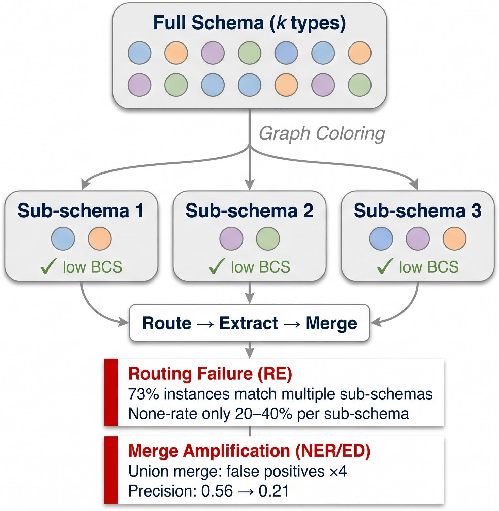
\includegraphics[width=\columnwidth]{../../figures/paper/fig_sdgd_pipeline_compact.pdf}
\caption{Schema decomposition pipeline and failure modes. Graph coloring partitions the schema into low-confusability sub-schemas, but two structural bottlenecks prevent practical gains: \textbf{routing failure} in RE (73.4\% of instances match multiple sub-schemas) and \textbf{merge amplification} in NER/ED (union merge increases false positives ${\sim}4\times$).}
\label{fig:sdgd_pipeline}
\end{figure}

\begin{table}[t]
\centering
\small
\caption{Routing strategy comparison on FewRel 80-relation RE with graph-coloring sub-schema decomposition. Oracle requires gold labels. All practical strategies perform below the single-pass baseline due to constrained decoding: 73.4\% of instances match multiple sub-schemas simultaneously.}
\label{tab:routing_strategies}
\resizebox{\columnwidth}{!}{\begin{tabular}{@{}lrr@{}}
\toprule
\textbf{Strategy} & \textbf{Accuracy} & \textbf{$\Delta$ vs.\ Single-Pass} \\
\midrule
Oracle (gold label) & 72.4\% & +22.0\,pp \\
\midrule
Max-conf (positive only) & 36.5\% & $-$14.0\,pp \\
None-aware & 36.5\% & $-$14.0\,pp \\
Margin (positive only) & 35.9\% & $-$14.5\,pp \\
Max-conf (all) & 27.7\% & $-$22.7\,pp \\
Random & 14.7\% & $-$35.7\,pp \\
\midrule
Single-pass (no decomposition) & 50.4\% & --- \\
\bottomrule
\end{tabular}}
\end{table}

\looseness=-1
A natural intervention is to partition the schema so confusable types never co-occur (Figure~\ref{fig:sdgd_pipeline}). We tested Schema-DAG-Guided Decomposition (SDGD), which applies greedy graph coloring on the SCS graph to assign types to low-confusability batches. While oracle routing recovers accuracy (0.724 vs.\ 0.504 single-pass; Table~\ref{tab:routing_strategies}), all practical routing strategies fall below the single-pass baseline, and NER decomposition amplifies false positives (F1: 0.445$\to$0.251). Merge amplification is the structural bottleneck: union merge increases false positives ${\sim}4\times$ (precision: 0.56$\to$0.21) while voting merge sacrifices recall. Confusability-aware batch composition avoids routing entirely and achieves higher accuracy under oracle assignment (Appendix~\ref{sec:appendix_batch_composition}). Full protocol and routing strategy evaluation in Appendix~\ref{sec:appendix_sdgd}.


\section{Discussion and Conclusion}
\label{sec:discussion}

\looseness=-1
\textbf{RQ1} (independent confusability effect): Yes, on RE. BCS independently explains ${\sim}$27\% of cross-batch accuracy variance on FewRel after controlling for count and centrality, replicating across three model scales. The NER null reflects dispersed error modes rather than absence of confusability effects (\S\ref{sec:multi_channel}).
\textbf{RQ2} (degradation modes): Count reduces recall overall (monotonically in RE; non-monotonically in NER); confusability drives type substitution (IntraSub) that scales monotonically with BCS. The two dimensions interact with bounded magnitude on the linear scale.
\textbf{RQ3} (decomposition): Schema decomposition fails in practice due to routing ambiguity (RE) and merge amplification (NER/ED), though oracle routing confirms the dimensions are separable in principle (\S\ref{sec:sdgd}).

\begin{table}[t]
\centering
\small
\caption{Intra-batch substitution (IntraSub) and missed rates by BCS bin. IntraSub scales monotonically with BCS across all three datasets. DocRED missed rates decrease with BCS, indicating errors shift from omission to substitution.}
\label{tab:error_taxonomy}
\resizebox{\columnwidth}{!}{%
\begin{tabular}{llrrrrrrr}
\toprule
 & & \multicolumn{5}{c}{\textbf{BCS Bin}} & & \\
\cmidrule(lr){3-7}
\textbf{Task} & \textbf{Error} & \textbf{Solo} & \textbf{Low} & \textbf{Mid} & \textbf{High} & \textbf{V.High} & \textbf{$\rho$} & \textbf{$p$} \\
\midrule
NER & IntraSub & 0\% & 1.6\% & 10.6\% & 49.4\% & --- & 1.000 & ${<}0.001$ \\
RE  & IntraSub & 0\% & 4.2\% & 13.0\% & 20.3\% & 32.3\% & 0.954 & ${<}\,0.001$ \\
DocRED & IntraSub & --- & 4.8\% & 22.4\% & 37.0\% & 41.9\% & 0.843 & ${<}\,0.001$ \\
\midrule
NER & Missed & --- & 42.8\% & 64.8\% & 49.9\% & --- & --- & --- \\
RE  & Missed & --- & 10.4\% & 11.3\% & 13.1\% & 15.7\% & --- & --- \\
DocRED & Missed & --- & 28.1\% & 22.6\% & 21.6\% & 16.2\% & --- & --- \\
\bottomrule
\end{tabular}}
\end{table}


\looseness=-1
We hypothesize that near-neighbor types in embedding space activate overlapping LLM representations, producing type-substitution interference consistent with ecological confusability \citep{baan-2023-ecological}, explaining why BCS predicts RE accuracy but not NER F1 (where errors concentrate in span boundary and missed-entity modes). The signal applies to cross-domain schemas; same-domain schemas exhibit centrality confounding (\S\ref{sec:centrality_confound}). For practitioners, reducing candidate types is the primary lever for NER; for RE, pre-computing SCS/BCS can flag high-risk schemas before deployment. Naive mitigations (renaming, few-shot) do not close the gap (Appendices~\ref{app:renaming},~\ref{sec:appendix_fewshot_bcs}). Probing the representational mechanism remains future work.


\section*{Limitations}
\looseness=-1
\textbf{(1)~Model scope.}
Primary experiments use Qwen3-32B; cross-model validation covers count and BCS but not secondary analyses. All evidence is correlational.
\textbf{(2)~DocRED multicollinearity.}
Severe VIF (50.9) prevents reliable BCS quantification; semipartial $R^2{}\,=\,5.6\%$ is directional only.
\textbf{(3)~Experimental scope.}
Four English Wikipedia/Wikidata datasets in a zero-shot setting; few-shot, fine-tuned, and non-English scenarios remain untested. BCS predicts RE accuracy but not NER. Cross-dataset consistency is converging evidence, not independent replication \citep{rothman-1990}.

\section*{Ethical Considerations}
This work is a controlled empirical analysis of schema complexity effects on training-free LLM information extraction. All datasets used (Few-NERD, FewRel, DocRED, MAVEN) are publicly available and derived from Wikipedia/Wikidata. No new data was collected, no human subjects were involved, and no crowd-sourced annotation was performed. Our findings characterize when LLMs fail under complex schemas, which may help practitioners identify high-risk deployment scenarios before committing resources.

% \section*{Responsible NLP Research Checklist}

For each question, the answer is \textbf{Yes}, \textbf{No}, or \textbf{N/A}. If Yes, the relevant section is indicated. If No, a justification is provided.

\subsection*{A \quad For Every Submission}

\begin{enumerate}[label=\textbf{A\arabic*.},leftmargin=*,itemsep=4pt]

\item \textbf{Did you describe the limitations of your work?}

Yes. The Limitations section (after \S\ref{sec:discussion}) discusses model coverage, effect size and statistical design (including TOST equivalence), task scope, causal mechanism, data contamination, and domain/language scope.

\item \textbf{Did you discuss any potential risks of your work?}

Yes (Limitations). SCS/BCS may be misused as a standalone deployment criterion. Since they are proxies for confusability and do not capture domain-specific ambiguity or downstream harms, they should be used for diagnostic monitoring rather than automatic schema rejection or high-stakes deployment decisions.

\item \textbf{Do the abstract and introduction summarize the paper's main claims?}

Yes. The abstract and \S\ref{sec:introduction} state the two-dimensional degradation pattern (count and confusability), the cross-model consistency check, and the negative SDGD result.

\item \textbf{Did you use AI assistants (e.g., ChatGPT, Copilot) when working on this paper?}

Yes. We used Claude (Anthropic) for writing assistance and experimental code development. All scientific claims, experimental designs, and analyses were conducted by the authors.

\end{enumerate}

\subsection*{B \quad Scientific Artifacts}

\begin{enumerate}[label=\textbf{B\arabic*.},leftmargin=*,itemsep=4pt]

\item \textbf{Did you cite the creators of artifacts you used?}

Yes. Few-NERD \citep{fewnerd-2021}, FewRel \citep{fewrel-2018}, DocRED \citep{docred-2019}, MAVEN \citep{maven-2020}, Qwen3-32B \citep{qwen3-2025}, Meta-Llama-3.1-70B-Instruct and Meta-Llama-3.1-8B-Instruct \citep{llama3-2024}, Gemini 2.5 Flash \citep{gemini-2025}, vLLM \citep{vllm-2023}, and all-MiniLM-L6-v2 \citep{minilm-2020} are cited in \S\ref{sec:datasets} and \S\ref{sec:model}.

\item \textbf{Did you discuss the license or terms for use and/or distribution of any artifacts?}

Yes. All four datasets are publicly available research benchmarks. Few-NERD is released under CC-BY-SA 4.0; FewRel, DocRED, and MAVEN are publicly released for research use. Open-weight models are used under their respective licenses; Gemini 2.5 Flash is accessed via the Google API under its terms of service.

\item \textbf{Did you discuss if your use of existing artifacts is consistent with their intended use?}

Yes. All datasets are used for their intended purpose (IE evaluation). No data is used outside the scope specified by the dataset creators.

\item \textbf{Did you discuss whether the data contains personally identifiable information or offensive content?}

N/A. We use established benchmarks that have been vetted by the research community. No new data collection or annotation was performed.

\item \textbf{Did you provide documentation of the artifacts, e.g., coverage of languages, coverage of domains, etc.?}

Yes. Table~\ref{tab:datasets} reports type counts, evaluation unit counts, domain characteristics, and BCS ranges for each dataset. \S\ref{sec:datasets} describes dataset provenance and sampling procedures.

\item \textbf{Did you report relevant statistics for your dataset(s)?}

Yes. \S\ref{sec:datasets} and Table~\ref{tab:datasets} report evaluation set sizes, type counts, and sampling methodology. Count levels and batch sizes are specified in \S\ref{sec:exp_design}.

\end{enumerate}

\subsection*{C \quad Computational Experiments}

\begin{enumerate}[label=\textbf{C\arabic*.},leftmargin=*,itemsep=4pt]

\item \textbf{Did you report the number of parameters in the models used, the total computational budget, and computing infrastructure?}

Yes. \S\ref{sec:model}: Qwen3-32B (32B parameters, FP8), Meta-Llama-3.1-70B-Instruct (70B parameters, FP8), and Meta-Llama-3.1-8B-Instruct (8B parameters). Gemini 2.5 Flash was additionally accessed via API for cross-architecture validation. Inference was conducted on NVIDIA RTX PRO 6000 GPUs (96\,GB) served via vLLM. Total compute was approximately 72 GPU-hours of inference (no training).

\item \textbf{Did you discuss the experimental setup, including hyperparameter search and best-found values?}

Yes. \S\ref{sec:exp_design} describes both experimental paradigms (count curves and BCS-controlled). \S\ref{sec:model} reports decoding parameters (greedy, temperature${}=0$, seed${}=42$) and prompt versions. No hyperparameter search was conducted as this is a zero-shot evaluation study.

\item \textbf{Did you report descriptive statistics about your results?}

Yes. All key metrics include 95\% bootstrap confidence intervals (10{,}000 resamples, percentile method) as stated in \S\ref{sec:model}. Spearman correlations are reported with $p$-values throughout \S\ref{sec:count_curves}--\ref{sec:centrality_confound}. Permutation tests are used for slope comparisons.

\item \textbf{Did you report implementation details, e.g., versions of packages?}

Yes. \S\ref{sec:model} specifies vLLM v0.20.2 for model serving. Embedding models are named with version identifiers (\S\ref{sec:scs}). Code and scripts are available at \url{https://anonymous.4open.science/r/schema-dag-extraction-4C10/}.

\end{enumerate}

\subsection*{D \quad Human Annotators or Crowdworkers}

\begin{enumerate}[label=\textbf{D\arabic*.},leftmargin=*,itemsep=4pt]

\item \textbf{Did you report the full text of instructions given to participants?}

N/A. No human annotation or crowdsourcing was conducted.

\item \textbf{Did you report information about how you recruited and paid participants?}

N/A.

\item \textbf{Did you discuss whether and how consent was obtained?}

N/A.

\item \textbf{Did you report whether the data collection was approved by an institutional review board (IRB)?}

N/A.

\item \textbf{Did you report the basic demographic and geographic characteristics of the annotator population?}

N/A.

\end{enumerate}

\subsection*{E \quad AI-Assisted Research}

\begin{enumerate}[label=\textbf{E\arabic*.},leftmargin=*,itemsep=4pt]

\item \textbf{Did you report the use of AI assistants?}

Yes. See A4 above. AI assistants were used for code development and document formatting. The research design, execution, and interpretation are the authors' own work.

\end{enumerate}
  % EMNLP 2026: checklist goes in OpenReview form, not PDF

\bibliography{references}

\appendix

\section{Additional Figures}
\label{sec:appendix_figures}

\begin{table}[h]
\centering
\small
\caption{Cross-model count-curve replication on Few-NERD (text-match recall). Both models show a general declining trend in recall with schema size. Per-batch correlation $r = 0.725$. Qwen3-32B values use the v2 prompt (\S\ref{sec:model}) for fair cross-model comparison; the count-curve results in \S\ref{sec:count_curves} use the v1 prompt, yielding higher absolute recall (0.72 vs.\ 0.64 at count${}\,=\,1$) due to over-prediction under v1.}
\label{tab:cross_model}
\begin{tabular}{lrr}
\toprule
\textbf{Count} & \textbf{Llama-3.1-8B} & \textbf{Qwen3-32B} \\
\midrule
1 & 0.702 & 0.640 \\
64 & 0.273 & 0.304 \\
\midrule
Decline & $-$43\,pp & $-$34\,pp \\
\bottomrule
\end{tabular}
\end{table}

\begin{table}[h]
\centering
\small
\caption{Cross-model BCS-controlled FewRel accuracy.  High-BCS accuracy converges to $\approx$51\% regardless of model, while low-BCS accuracy reflects model capacity differences.  The confusability gap ($\Delta$, in pp) is 77--87\% as large on Llama-3.1-8B as on Qwen3-32B.}
\label{tab:cross_model_bcs}
\resizebox{\columnwidth}{!}{%
\begin{tabular}{crrrrrr}
\toprule
& \multicolumn{3}{c}{\textbf{Llama-3.1-8B}} & \multicolumn{3}{c}{\textbf{Qwen3-32B}} \\
\cmidrule(lr){2-4} \cmidrule(lr){5-7}
\textbf{Count} & \textbf{Low} & \textbf{High} & \textbf{$\Delta$} & \textbf{Low} & \textbf{High} & \textbf{$\Delta$} \\
\midrule
8 & 78.1\% & 51.0\% & $-$27.1 & 82.3\% & 51.0\% & $-$31.2 \\
16 & 75.5\% & 51.6\% & $-$23.9 & 82.8\% & 51.6\% & $-$31.2 \\
\bottomrule
\end{tabular}}
\end{table}

\begin{table}[h]
\centering
\small
\caption{NER batch-level BCS--F1 correlation across models. $^\dagger$Partial correlation controlling for type frequency. $^\ddagger$Llama-70B count\_12 shows $r{=}{-}0.42$ ($p{=}0.034$, uncorrected; Bonferroni $p{=}0.069$); pooled and count\_6 are null, consistent with sampling noise at $n{=}25$. The null is observed on three models; Gemini remains untested.}
\label{tab:cross_model_ner_null}
\begin{tabular}{lcl}
\toprule
\textbf{Model} & \textbf{NER BCS--F1 $r$} & \textbf{Status} \\
\midrule
Qwen3-32B & $0.004$ ($p = 0.94$) & Null \\
Llama-3.1-8B & $-0.12$ ($p = 0.29$)\rlap{$^\dagger$} & Null \\
Llama-3.1-70B & $-0.13$ ($p = 0.36$)\rlap{$^\ddagger$} & Null \\
Gemini 2.5 Flash & --- & Not tested \\
\bottomrule
\end{tabular}
\end{table}

Table~\ref{tab:error_taxonomy} (in \S\ref{sec:multi_channel}) reports IntraSub and missed rates by BCS bin.

\begin{table}[t]
\centering
\small
\caption{Cross-model replication of IntraSub--BCS Spearman correlation on FewRel RE. $^\dagger$Llama-70B has only 20 batches with 17.4\% missed rate; the null is attributable to insufficient power rather than absence of the effect.}
\label{tab:cross_model_error_taxonomy}
\begin{tabular}{lrcc}
\toprule
\textbf{Model} & $n$ & $\rho$ & $p$ \\
\midrule
Qwen3-32B & 154 & 0.954 & ${<}\,0.001$ \\
Gemini 2.5 Flash & 60 & 0.821 & ${<}\,0.001$ \\
Llama-3.1-8B & 54 & 0.430 & 0.001 \\
Llama-3.1-70B$^\dagger$ & 20 & $-$0.086 & 0.719 \\
\bottomrule
\end{tabular}
\end{table}

\section{SDGD Full Protocol and Results}
\label{sec:appendix_sdgd}

We construct a thresholded confusability graph $G = (V, E)$ where each type is a vertex and an edge connects types $t_i, t_j$ whenever $\text{SCS}(t_i, t_j) > \tau$. Greedy graph coloring (\textsc{largest\_first}) assigns each type to a color such that no two adjacent (i.e., highly confusable) types share a color. Each color class forms one extraction batch, and predictions are merged via set union.

\begin{enumerate}[leftmargin=*,itemsep=2pt]
\item Compute pairwise SCS matrix $S_{ij} = \cos(\text{embed}(t_i), \text{embed}(t_j))$.
\item Construct graph $G$: add edge $(t_i, t_j)$ iff $S_{ij} > \tau$.
\item Apply greedy graph coloring (\textsc{largest\_first}) to assign each type a color $c(t)$.
\item For each color $k$, form batch $B_k = \{t : c(t) = k\}$ and run extraction on all test instances.
\item Merge: union of per-batch predictions (v1) or confidence-gated selection (v2).
\end{enumerate}
Oracle routing (Table~\ref{tab:routing_strategies}) recovers substantial accuracy (72.4\% vs.\ 50.4\% single-pass), confirming the sub-schemas contain correct predictions; the failure lies in routing, not decomposition quality.

We compare four modes: (i)~\textbf{single\_pass}, the undecomposed baseline; (ii)~\textbf{sdgd\_zero}, SCS-guided partitioning; (iii)~\textbf{random\_batch}, random partitioning with matched batch sizes; and (iv)~\textbf{per\_type}, the extreme case where each type is extracted in isolation.

Single-pass extraction achieves F1\,=\,0.445 (P\,=\,0.563, R\,=\,0.368). SDGD obtains F1\,=\,0.251 (P\,=\,0.210, R\,=\,0.314), a 44\% relative drop. Random batching reaches F1\,=\,0.320 (P\,=\,0.249, R\,=\,0.446), and per-type extraction yields F1\,=\,0.292 (P\,=\,0.194, R\,=\,0.586). Every decomposition mode falls below the single-pass baseline (Table~\ref{tab:sdgd_results}).

\begin{table}[h]
\centering
\small
\caption{Few-NERD extraction under decomposition modes. V1 uses union merge; v2 uses confidence-gated merge with \texttt{min\_batch\_size=8} (reducing 8$\to$4 batches for sdgd\_zero). All decomposition modes produce lower F1 than the single-pass baseline. All modes use the v1 prompt.}
\label{tab:sdgd_results}
\resizebox{\columnwidth}{!}{%
\begin{tabular}{lrccc}
\toprule
\textbf{Mode} & \textbf{\# Batches} & \textbf{Precision} & \textbf{Recall} & \textbf{F1} \\
\midrule
single\_pass & 1 & 0.563 & 0.368 & 0.445 \\
\midrule
sdgd\_zero (v1) & 8 & 0.210 & 0.314 & 0.251 \\
random\_batch (v1) & 8 & 0.249 & 0.446 & 0.320 \\
per\_type & 66 & 0.194 & 0.586 & 0.292 \\
\midrule
sdgd\_zero (v2) & 4 & 0.324 & 0.191 & 0.241 \\
random\_batch (v2) & 8 & 0.331 & 0.276 & 0.301 \\
\bottomrule
\end{tabular}}
\end{table}

Decomposition boosts recall (per-type recall reaches 0.586 versus single-pass 0.368) but devastates precision (0.194 versus 0.563). When the same text is presented to the model $k$ times with different type subsets, each pass independently generates entity predictions. Because LLM outputs are not calibrated across passes, the union merge step accumulates overlapping and contradictory predictions and inflates false positives.

Our v2 merge ranks competing predictions by the LLM's self-reported confidence and retains only the highest-scoring candidate for each span. Confidence gating improves precision (sdgd\_zero: 0.210$\to$0.324; random\_batch: 0.249$\to$0.331), but at the cost of disproportionate recall loss (0.314$\to$0.191; 0.446$\to$0.276), and both modes produce lower F1 (sdgd\_zero: 0.251$\to$0.241; random\_batch: 0.320$\to$0.301).

\subsection{Practical Routing Strategies on RE}
\label{sec:appendix_routing}

We evaluate five non-oracle routing strategies on FewRel 80-relation RE using graph-coloring sub-schema decomposition (same grouping as Table~\ref{tab:batch_composition}). Each strategy selects a single sub-schema for each test instance and returns that sub-schema's prediction.

Table~\ref{tab:routing_strategies} (in \S\ref{sec:sdgd}) summarizes routing strategy results.

\section{Factorial Analysis and Separability Test}
\label{sec:appendix_factorial}

To formally test whether count and confusability effects are additive, we fit a multiple regression (accuracy $\sim$ $\log_2$\,count $+$ BCS $+$ count$\times$BCS) across 69 batches from FewRel spanning five count levels ($k \in \{4, 8, 16, 32, 40\}$). Both main effects are significant (count: $p = 0.008$; BCS: $p = 0.0002$; $R^2 = 0.52$), but the interaction term is negligible (0.47\,pp). A TOST equivalence test with a $\pm 3$\,pp margin confirms that the interaction is bounded well below practical significance ($p_{\text{TOST}} = 0.003$); this supports bounded interaction between count and confusability effects.

A $2 \times 2$ factorial sensitivity check on FewRel (count $\in \{8, 16\}$, BCS low/high; $n = 54$) was inconclusive ($p_{\text{TOST}} = 0.56$) due to limited power; this does not contradict the primary finding but limits generalization beyond the regression framework. The Few-NERD factorial (\S\ref{sec:multi_channel}) similarly did not reach significance ($p = 0.50$). The regression approach provides the stronger test by leveraging the full count range.

\paragraph{Equivalence margin justification.}
We set the $\pm 3$\,pp margin based on three converging anchors. \emph{External}: evaluation variance in IE benchmarks typically spans 2--5\,pp across random seeds, prompt variations, and data splits \citep{card-2020-power,dror-2018-significance}; our own four structurally distinct prompt variants yield cross-variant accuracy SD of 3.5--4.6\,pp across count conditions (Table~\ref{tab:prompt_variants}), confirming that a within-margin interaction would be indistinguishable from routine prompt-design noise and satisfying the smallest-effect-of-interest criterion \citep{lakens-2017-equivalence}. \emph{Internal}: $0.5 \times$ within-cell SD ($= 2.3$\,pp) corresponds to Cohen's $d \approx 0.5$ (medium effect threshold; \citealt{lakens-2017-equivalence}), cross-validated against the IQR-predicted confusability main effect of 2.2\,pp (\S\ref{sec:practical_magnitude})---an interaction exceeding 3\,pp would represent ${>}130\%$ amplification. \emph{Sensitivity}: Table~\ref{tab:tost_sensitivity} shows equivalence holds from $\pm 2$\,pp ($p = 0.047$) through $\pm 5$\,pp ($p < 0.001$) on the probability scale; the conclusion is not margin-dependent.

\begin{table}[h]
\centering
\small
\caption{TOST sensitivity analysis across equivalence margins. The interaction effect (0.47\,pp, 90\% CI [$-$1.0, 2.0]\,pp) is bounded below 2\,pp at marginal significance ($p = 0.047$); the $\pm 3$\,pp choice does not drive the equivalence conclusion. At $\pm 1$\,pp, equivalence is inconclusive ($p = 0.278$), meaning interaction could reach approximately half the main effect magnitude.}
\label{tab:tost_sensitivity}
\begin{tabular}{crrl}
\toprule
\textbf{Margin (pp)} & \textbf{$t_{\text{upper}}$} & \textbf{$p_{\text{TOST}}$} & \textbf{Conclusion} \\
\midrule
$\pm 1$ & $-0.59$ & $0.278$ & Inconclusive \\
$\pm 2$ & $-1.70$ & $0.047$ & Equivalent \\
$\pm 3$ & $-2.81$ & $0.003$ & Equivalent \\
$\pm 5$ & $-5.02$ & ${<}\,0.001$ & Equivalent \\
\bottomrule
\end{tabular}
\end{table}

\paragraph{Logit-scale sensitivity.}
Because accuracy near 50\% compresses interaction effects on the linear scale, we refit the regression on logit-transformed accuracy. The logit-scale interaction (0.111 logit units, $p = 0.047$, 90\% CI [0.019, 0.203]) is marginally significant, and TOST at the equivalent $\pm 3$\,pp margin ($\pm 0.156$ logit at median accuracy) is inconclusive ($p_{\text{TOST}} = 0.209$). However, back-transforming the interaction to the probability scale at the observed floor ($p = 0.51$) yields 2.78\,pp, still within the $\pm 3$\,pp margin; at the median baseline ($p = 0.65$), the back-transformed effect is 2.53\,pp. The logit TOST is inconclusive due to limited power ($n = 69$, wide CI) rather than a large effect size: the point estimate remains below the equivalence bound at all observed baselines. We retain the linear-scale TOST as the primary test and report this logit analysis as a sensitivity check. A regression-based TOST ($n = 375$, five count levels with continuous BCS) yields $p = 0.050$ at $\pm 3$\,pp and $p = 0.026$ at $\pm 3.5$\,pp on the logit scale, confirming the borderline status with substantially greater power than the factorial design.

\paragraph{DocRED factorial (expanded).}
With expanded batches ($n{=}55$ per count level, up from $n{=}5$), the DocRED $2 \times 2$ factorial (count $\in \{16, 32\}$, BCS median split) yields an apparent interaction ($-$9.4\,pp, 95\% CI [$-$12.9, $-$6.0]): the BCS effect is $-$25.0\,pp at count 16 but $-$15.7\,pp at count 32. However, this attenuation is confounded by BCS range restriction: higher-count batches have narrower BCS ranges (spread 0.26 vs.\ 0.38), limiting achievable extremes.

\paragraph{Range-matched robustness check.}
To control for the BCS range confound, we restrict both count levels to the overlapping BCS range [0.43, 0.70]. This retains 29 of 55 batches at count 16 (all 55 at count 32 fall within the range). Within this matched range, the BCS effect at count 16 shrinks from 15.95\,pp to 9.37\,pp (reflecting the narrower BCS span), while count 32 remains at 8.44\,pp. The interaction drops from 7.52\,pp (95\% CI [1.49, 12.83]) to 0.93\,pp (95\% CI [$-$7.13, 7.44])---the CI spans zero, consistent with no interaction. Spearman correlations remain comparable ($\rho = -0.65$ at count 16, $\rho = -0.69$ at count 32), confirming that the underlying BCS--accuracy relationship is robust across counts while the raw interaction magnitude was an artifact of differing achievable BCS ranges. This result aligns with the FewRel TOST equivalence finding and supports bounded association as the cross-dataset pattern. The reduced sample ($n = 29{+}55$) yields a minimum detectable effect of 5.5\,pp at 80\% power, consistent with insufficient power to distinguish a true null from a small ($<$5\,pp) interaction.

\section{Within-Pool CI Details}
\label{sec:appendix_within_pool}

The quartile $\Delta$ for 80-pool 16-relation subsets ($-$3.92\,pp, 95\% CI [$-$8.17, $+$0.38]) crosses zero, reflecting the compressed BCS range within that pool (0.46--0.68 vs.\ 0.48--0.71 for the independent pool). Within this narrow band, the quartile contrast lacks statistical power to detect the effect that the regression identifies. The full 80-relation condition ($n = 25$) is underpowered for both the slope (95\% CI [$-$1.303, $+$1.695]) and quartile analyses; we include it in Table~\ref{tab:within_pool} for completeness but do not draw inferential conclusions from it.

\section{Controlling for Centrality Confounds in MAVEN Per-Type Analysis}
\label{sec:appendix_residualized_bcs}

Section~\ref{sec:centrality_confound} identifies a centrality confound in MAVEN's per-type BCS--F1 correlation: both embeddings show a \emph{positive} raw correlation, opposite to the expected direction. Here we formalize this analysis by identifying specific confounders for each embedding and testing whether the BCS--F1 relationship survives partial correlation controlling for these confounders.

\paragraph{Confound identification.}
For each embedding, we computed the correlation between mean BCS and candidate confounders (type frequency, degree centrality at threshold 0.7) across MAVEN's 149 active event types. The dominant confound differs by embedding:
\begin{itemize}[itemsep=2pt,leftmargin=*]
\item \textbf{MiniLM}: BCS correlates with log type frequency ($r = 0.201$). Frequent types have more training signal and are extracted more reliably, which produces the positive BCS--F1 association.
\item \textbf{Qwen3}: BCS correlates strongly with degree centrality ($r = 0.854$). In the Qwen3 embedding space, high-BCS types are those with many semantic neighbors, central, well-represented types that the model extracts well.
\end{itemize}

\paragraph{Partial correlation results.}
Table~\ref{tab:residualized_bcs} reports raw Spearman $\rho$ and partial Pearson $r$ after controlling for the identified confounders. Under single-variable control, both correlations weaken to non-significance. Under joint control (log frequency $+$ degree centrality simultaneously), neither embedding retains a significant BCS--F1 association.

\begin{table}[h]
\centering
\small
\caption{MAVEN per-type BCS--F1 correlation before and after controlling for centrality confounders. Raw correlations are Spearman $\rho$; partial correlations are Pearson $r$ from residualized regression. Degree centrality is computed on the SCS graph at threshold 0.7. All values from the residualized BCS analysis.}
\label{tab:residualized_bcs}
\resizebox{\columnwidth}{!}{%
\begin{tabular}{llcccc}
\toprule
\textbf{Embedding} & \textbf{Control} & \textbf{Raw $\rho$} & \textbf{Raw $p$} & \textbf{Partial $r$} & \textbf{Partial $p$} \\
\midrule
MiniLM & --- & $+$0.208 & $0.011$ & --- & --- \\
MiniLM & log freq & --- & --- & $+$0.133 & $0.11$ \\
MiniLM & log freq $+$ degree & --- & --- & --- & $0.23$ \\
\midrule
Qwen3 & --- & $+$0.184 & $0.025$ & --- & --- \\
Qwen3 & degree centrality & --- & --- & $+$0.063 & $0.44$ \\
Qwen3 & log freq $+$ degree & --- & --- & --- & $0.44$ \\
\bottomrule
\end{tabular}}
\end{table}

\paragraph{Interpretation.}
The two embeddings encode different aspects of the same underlying confound. MiniLM, a smaller sentence encoder, produces a tighter embedding cluster for MAVEN's FrameNet-derived types; here, type frequency is the primary confounder because frequent types accumulate higher mean similarity to the dense cluster. Qwen3, with a larger representation space, differentiates types enough that frequency is not the dominant factor, but degree centrality (the count of strong semantic neighbors) becomes the confound instead. In both cases, the positive raw correlation reflects a centrality artifact: types that are semantically central are both high-BCS and easy to extract.

Under joint control, both embeddings yield $p > 0.2$; the raw positive BCS--F1 correlation on MAVEN is thus fully attributable to centrality-related confounders. This does not invalidate the confusability hypothesis; the pairwise SCS--confusion correlation on MAVEN remains significant (MiniLM $r = 0.129$, $p < 0.001$; Table~\ref{tab:pairwise}). Rather, it demonstrates that per-type aggregation (mean BCS) conflates confusability with centrality in semantically homogeneous schemas, and that pairwise analysis or explicit confound adjustment is required in such settings.

\subsection{Partial Correlation: Controlling for Degree Centrality}
\label{sec:appendix_partial_corr}

To rule out degree centrality as a confound in cross-domain datasets, we compute partial correlations between BCS and accuracy controlling for batch mean degree centrality (mean off-diagonal SCS per type, averaged across batch members).

\begin{table}[h]
\centering
\small
\caption{BCS--accuracy partial correlation controlling for degree centrality. FewRel shows minimal attenuation (VIF${}\,=\,1.18$, low collinearity). DocRED shows high BCS--centrality collinearity (VIF${}\,=\,50.9$, $r = 0.99$), but the partial correlation remains highly significant.}
\label{tab:partial_corr}
\begin{tabular}{lrrrrr}
\toprule
\textbf{Dataset} & \textbf{$n$} & \textbf{$r_{\text{zero}}$} & \textbf{$r_{\text{partial}}$} & \textbf{$p_{\text{partial}}$} & \textbf{VIF} \\
\midrule
FewRel & 204 & $-$0.570 & $-$0.537 & ${<}\,0.001$ & 1.18 \\
DocRED & 110 & $-$0.760 & $-$0.348 & ${<}\,0.001$ & 50.9 \\
\bottomrule
\end{tabular}
\end{table}

As Table~\ref{tab:partial_corr} shows, on FewRel, BCS and degree centrality are only moderately correlated ($r = 0.39$), and the BCS effect survives nearly intact after partialling ($r_{\text{partial}} = -0.537$ vs.\ $r_{\text{zero}} = -0.570$; semipartial $R^2 = 0.273$). On DocRED, the near-perfect BCS--centrality correlation ($r = 0.99$) makes it impossible to fully separate the two predictors; the significant partial correlation ($p < 0.001$) indicates BCS retains predictive value but does not uniquely identify the causal channel. This contrasts with MAVEN (\S\ref{sec:appendix_residualized_bcs}), where the BCS signal vanishes after controlling for centrality.

\paragraph{Ridge regression under multicollinearity.}
Ridge regression (GCV, $\lambda = 0.001$) on the 110 DocRED batches confirms the negative direction of the BCS--accuracy relationship even after regularizing for the severe BCS--centrality multicollinearity (VIF$\,\approx\,$50.9). The standardized BCS coefficient is $\hat{\beta}_{\text{BCS}} = -1.53$ ($\hat{\beta}_{\text{centrality}} = 0.78$, $R^2 = 0.594$). An analytic derivation shows that $\hat{\beta}_{\text{BCS}} < 0$ for \emph{all} $\lambda \geq 0$: the numerator of the closed-form ridge solution, $-(1{+}\lambda) \times 0.760 + 0.727$, is negative at $\lambda{=}0$ and monotonically decreasing thereafter. Given the shrinkage bias inherent to ridge estimation, we interpret only the sign---not the magnitude---of the BCS coefficient as directional evidence that higher schema confusability degrades extraction accuracy, independent of degree centrality.

\subsection{NER BCS-Null Power Analysis}
\label{sec:appendix_ner_power}

The Few-NERD BCS-null may reflect insufficient BCS variance rather than a genuine absence of the BCS--accuracy relationship. Few-NERD's BCS standard deviation (0.027) is only 19\% of FewRel's (0.141); FewRel's observed $r = -0.570$ would attenuate to $r = -0.111$ under this restricted range, yielding 65\% power at $n = 450$ (below the conventional 80\% threshold). The minimum detectable $|r|$ at 80\% power is 0.132. This analysis characterizes the NER result as absence of evidence (insufficient power at the attenuated effect size) rather than evidence of absence.

\subsection{Bootstrap CI Robustness}
\label{sec:appendix_bootstrap_ci}

Because batches in the FewRel experiments are constructed by sampling relation types from a shared pool, different batches may share text instances of the same type, potentially inducing residual dependence that makes standard bootstrap CIs anti-conservative. We assess this concern via cluster-robust inference. We cluster the $n = 164$ FewRel batches by instance-weighted type overlap (hierarchical clustering, complete linkage) and compute cluster-robust standard errors. Across six overlap thresholds (Jaccard distance $\in \{0.1, \ldots, 0.9\}$, yielding 80--83 clusters), the cluster-robust SE for the BCS regression slope is $0.96$--$0.97\times$ the OLS SE, and the slope remains highly significant ($p < 10^{-11}$). Cluster bootstrap CIs for $R^2$ show width changes of $-6\%$ to $+6\%$ relative to standard bootstrap CIs ($[0.14, 0.42]$ vs.\ $[0.15, 0.41]$). We conclude that the reported CIs are robust to the non-independence induced by shared text instances.

\subsection{Domain Distribution in Extreme-BCS Batches}
\label{sec:appendix_domain_distribution}

We classify the 80 FewRel relation types into six semantic domains (geography, creative work, person, organization, event/temporal, science/taxonomy) and compare domain composition between the 25 highest-BCS and 25 lowest-BCS batches from our 8-type schema pool. The distributions differ significantly ($\chi^2 = 230.74$, $p < 0.001$, $df = 5$): low-BCS batches draw heavily from geography (45.5\%) and creative work (25.5\%), while high-BCS batches concentrate on science/taxonomy (49.5\%) and event/temporal (26.0\%) domains. Normalized Shannon entropy is higher for low-BCS batches ($H' = 0.79$) than high-BCS ($H' = 0.67$), confirming that low-BCS schemas span more diverse domains. Crucially, this domain concentration is an \emph{expected} property of embedding-based confusability: relation types within the same domain naturally share semantic features, producing higher pairwise cosine similarity and thus higher BCS. Domain composition therefore acts as a mediator---it is \emph{part of} the mechanism through which BCS captures schema difficulty---rather than an independent confounding variable. The BCS metric intentionally aggregates such semantic overlap into a single predictive score.

\section{Batch Composition Results}
\label{sec:appendix_batch_composition}

\begin{table}[h]
\centering
\small
\caption{Batch composition on FewRel 80-relation RE with oracle routing. $^\dagger$Mean $\pm$ SD across 15 random seeds.}
\label{tab:batch_composition}
\resizebox{\columnwidth}{!}{%
\begin{tabular}{@{}lcc@{}}
\toprule
\textbf{Condition} & \textbf{Accuracy} & \textbf{Mean BCS} \\
\midrule
Single-pass (80 types) & 0.504 & 0.557 \\
Random batching (15 seeds)$^\dagger$ & 0.788\,$\pm$\,0.018 & 0.559 \\
Confus.-aware (graph coloring) & \textbf{0.802} & 0.552 \\
\bottomrule
\end{tabular}}
\end{table}

See the accompanying discussion in \S\ref{sec:sdgd}.

\lstset{
  basicstyle=\ttfamily\small,
  breaklines=true,
  breakatwhitespace=true,
  columns=fullflexible
}

\section{Prompt Templates}
\label{sec:appendix_prompts}

This appendix reproduces the complete prompt templates used for all three extraction tasks.
All prompts are injected into a single \texttt{user} message (no system prompt); the model's chat template adds the system/assistant framing.
Both versions provide a JSON-formatted type schema to the vLLM constrained-decoding engine; the schema is \emph{not} included in the natural-language prompt itself.
We use greedy decoding (\texttt{temperature=0}, \texttt{seed=42}) throughout.

\medskip\noindent
\textbf{Notation.}
Placeholders are shown in \texttt{\{braces\}}.
Text \textbf{added in v2} (relative to v1) is marked with $\triangleright$.
Text \textbf{removed in v2} is marked with \sout{strikethrough}.

\subsection{Named Entity Recognition (Few-NERD)}

\paragraph{v1 prompt (with character offsets).}

\begin{small}
\begin{lstlisting}
Extract all named entities from the following text.
Only extract entities of the following types:
- {type_1}: {definition_1}
- {type_2}: {definition_2}
  ...

Text: {input_text}

Output as JSON: [{"text": "...", "type": "...",
                  "start": ..., "end": ...}]
\end{lstlisting}
\end{small}

\noindent
\textbf{v1 constrained-decoding schema:}
\begin{small}
\begin{lstlisting}
{"type": "array",
 "items": {"type": "object",
   "properties": {
     "text":  {"type": "string"},
     "type":  {"type": "string",
               "enum": [<sorted_types>]},
     "start": {"type": "integer"},
     "end":   {"type": "integer"}},
   "required": ["text","type","start","end"]}}
\end{lstlisting}
\end{small}

\paragraph{v2 prompt (text+type only).}

\begin{small}
\begin{lstlisting}
Extract all named entities from the following text.
Only extract entities of the following types:
- {type_1}: {definition_1}
- {type_2}: {definition_2}
  ...

Text: {input_text}
\end{lstlisting}
\end{small}
\vspace{-0.5em}
\noindent$\triangleright$~\textbf{Added in v2:}
\begin{small}
\begin{lstlisting}
Only extract entities that clearly match one of the
given types. If no entities of these types exist in
the text, output an empty list [].
\end{lstlisting}
\end{small}
\vspace{-0.5em}
\begin{small}
\begin{lstlisting}
Output as JSON: [{"text": "...", "type": "..."}]
\end{lstlisting}
\end{small}

\noindent
\textbf{v2 constrained-decoding schema:}
\begin{small}
\begin{lstlisting}
{"type": "array",
 "items": {"type": "object",
   "properties": {
     "text": {"type": "string"},
     "type": {"type": "string",
              "enum": [<sorted_types>]}},
   "required": ["text","type"]}}
\end{lstlisting}
\end{small}

\paragraph{v1 $\to$ v2 differences (NER).}
\begin{enumerate}[leftmargin=*,itemsep=2pt]
\item \textbf{Offset fields removed.} The \texttt{start}/\texttt{end} integer fields are dropped from both the natural-language instruction and the JSON schema. In v1, 96.5\% of predicted offsets were hallucinated (\S\ref{sec:model}).
\item \textbf{Format constraints added.} Two sentences are appended: (a)~``Only extract entities that clearly match one of the given types'' suppresses spurious predictions; (b)~``If no entities \ldots output an empty list~\texttt{[]}'' provides an explicit empty-output path.
\end{enumerate}

\subsection{Event Detection (MAVEN)}

\paragraph{v1 prompt (with character offsets).}

\begin{small}
\begin{lstlisting}
Extract all event triggers from the following text.
A trigger is the word or phrase that most clearly
expresses the event occurrence. Only extract triggers
of the following event types:
- {type_1}: {definition_1}
- {type_2}: {definition_2}
  ...

Text: {input_text}

Output as JSON: [{"text": "...", "type": "...",
                  "start": ..., "end": ...}]
\end{lstlisting}
\end{small}

\paragraph{v2 prompt (text+type only).}

\begin{small}
\begin{lstlisting}
Extract all event triggers from the following text.
A trigger is the word or phrase that most clearly
expresses the event occurrence. Only extract triggers
of the following event types:
- {type_1}: {definition_1}
- {type_2}: {definition_2}
  ...

Text: {input_text}
\end{lstlisting}
\end{small}
\vspace{-0.5em}
\noindent$\triangleright$~\textbf{Added in v2:}
\begin{small}
\begin{lstlisting}
Only extract triggers that clearly match one of the
given event types. If no events of these types exist
in the text, output an empty list [].
\end{lstlisting}
\end{small}
\vspace{-0.5em}
\begin{small}
\begin{lstlisting}
Output as JSON: [{"text": "...", "type": "..."}]
\end{lstlisting}
\end{small}

\noindent The JSON schemas for ED are identical to the NER schemas above; only the natural-language framing differs (``event triggers'' instead of ``named entities'').

\paragraph{v1 $\to$ v2 differences (ED).}
Same two changes as NER: offset fields removed, format constraints added.

\subsection{Relation Extraction (FewRel)}

RE uses only a v2-style prompt (no offset fields are applicable to classification).

\paragraph{Prompt.}

\begin{small}
\begin{lstlisting}
Given the following sentence and two entities,
classify the relation between them.

Sentence: "{sentence}"
Head entity: "{head_entity}"
Tail entity: "{tail_entity}"

Candidate relations: {type_1}, {type_2}, ...

Output a single JSON object:
  {"relation": "<relation_type>"}
If none of the candidate relations apply, output:
  {"relation": "none"}
\end{lstlisting}
\end{small}

\noindent
\textbf{Constrained-decoding schema:}
\begin{small}
\begin{lstlisting}
{"type": "object",
 "properties": {
   "relation": {"type": "string",
     "enum": [<sorted_types>, "none"]}},
 "required": ["relation"]}
\end{lstlisting}
\end{small}

\subsection{Type Definitions}
\label{sec:appendix_type_defs}

All prompts include per-type natural-language definitions sourced from the respective dataset documentation:
\begin{itemize}[leftmargin=*,itemsep=2pt]
\item \textbf{Few-NERD:} 66 fine-grained entity types with definitions derived from the Few-NERD type ontology \citep{fewnerd-2021}.
\item \textbf{MAVEN:} 168 event types with FrameNet-based definitions \citep{maven-2020}.
\item \textbf{FewRel:} 80 relation types with Wikidata property descriptions \citep{fewrel-2018}.
\end{itemize}

\noindent Type definitions are injected as ``\texttt{- \{type\_name\}: \{definition\}}'' lines in alphabetical order. The number of types per prompt varies by experimental condition (count${}= 1$ to full schema; \S\ref{sec:exp_design}).


\section{Prompt Version Sensitivity Analysis}
\label{sec:appendix_prompt_sensitivity}

We assess whether the confusability effects reported in \S\ref{sec:bcs_controlled}--\ref{sec:multi_channel} are robust to prompt design by replicating key experiments under the v2 prompt (\S\ref{sec:model}; full templates in Appendix~\ref{sec:appendix_prompts}).

\paragraph{RE (FewRel).}
Under the v1 prompt, the extreme-batch BCS gap (Table~\ref{tab:bcs_controlled}) is substantial. Under v2, with $n{=}25$ batches per group and wider BCS contrast (low-BCS range [0.356, 0.367]; high-BCS range [0.791, 0.811]), the gap is $-$25.5\,pp (low-BCS 85.2\% vs.\ high-BCS 59.7\%; 95\% CI [22.4, 28.6]; $p < 0.001$; Pearson $r = -0.919$). The effect is significant, directionally consistent with v1, and only modestly attenuated in magnitude ($-$5.7\,pp reduction). An earlier $n{=}5$ evaluation with narrower BCS contrast (0.21) yielded a smaller gap of $-$7.9\,pp (95\% CI [$-$5.2, $+$21.5]), illustrating how limited statistical power and restricted BCS range can obscure the underlying signal, a cautionary note for small-sample prompt sensitivity studies.

\paragraph{NER (Few-NERD).}
The batch-level BCS--F1 correlation is null under both prompt versions. Pooling across three seeds and all count levels ($n = 450$), the correlation is $r = 0.004$ ($p = 0.94$). An earlier small-sample analysis ($n = 27$, single seed) had reported positive correlations ($r = +0.50$/$+0.58$), but these were driven by an accidental BCS--type-frequency confound: those 27 batches exhibited $r(\text{BCS}, \text{freq}) = 0.53$, creating a spurious path through frequency to F1. After controlling for type frequency, the partial correlation is non-significant in both the small ($r = 0.28$, $p = 0.16$) and large ($r = -0.12$, $p = 0.29$) samples. The pairwise SCS--confusion analysis (\S\ref{sec:pairwise}), which is immune to this batch-level aggregation artifact, remains the primary evidence for the NER confusability dimension.

\paragraph{Interpretation.}
The $n{=}25$ v2 result confirms that the confusability effect is directionally consistent across prompt designs, with attenuated magnitude: the gap narrows ($-$5.7\,pp) but remains highly significant ($p < 0.001$, $r = -0.919$). The earlier $n{=}5$ non-significance reflected insufficient power and narrow BCS contrast, not absence of the effect. V2's stricter format constraints raise the baseline accuracy (low-BCS 85.2\% vs.\ 82.3\%), but type confusion under high confusability persists (59.7\% vs.\ 51.0\%). Prompt design modulates the practical magnitude of the confusability effect but does not eliminate it, ruling out prompt-specific confounding as the primary source. The underlying confusability signal (pairwise SCS--confusion correlation and the directional BCS--accuracy relationship) persists across both prompt versions.

\subsection{Cross-Prompt-Variant BCS Correlation}
\label{sec:appendix_prompt_variants}

To verify that the BCS--accuracy relationship is not an artifact of a specific prompt template, we evaluate four structurally distinct prompt variants on FewRel 80-relation RE at two count levels (8 and 32), with 10 random batches per condition (Table~\ref{tab:prompt_variants}).

\begin{table}[h]
\centering
\small
\caption{BCS--accuracy Pearson correlation across four prompt variants. At count 32, all four variants show negative BCS--accuracy correlations ($r \leq -0.47$), with two reaching $p < 0.05$. At count 8, the narrower BCS range reduces statistical power.}
\label{tab:prompt_variants}
\resizebox{\columnwidth}{!}{\begin{tabular}{lrrrr}
\toprule
\textbf{Variant} & \textbf{Count} & \textbf{Mean Acc} & \textbf{$r$} & \textbf{$p$} \\
\midrule
V2 (definition-first) & 8 & 0.769 & $-$0.333 & 0.348 \\
V2 (definition-first) & 32 & 0.564 & $-$0.648 & 0.043 \\
Instruction-rewrite & 8 & 0.847 & $-$0.223 & 0.536 \\
Instruction-rewrite & 32 & 0.662 & $-$0.469 & 0.171 \\
Chain-of-thought & 8 & 0.749 & $+$0.254 & 0.478 \\
Chain-of-thought & 32 & 0.617 & $-$0.566 & 0.088 \\
Minimal & 8 & 0.852 & $-$0.170 & 0.638 \\
Minimal & 32 & 0.615 & $-$0.771 & 0.009 \\
\bottomrule
\end{tabular}}
\end{table}

At count 32, all four variants produce negative BCS--accuracy correlations ($r$ ranges from $-$0.47 to $-$0.77), with V2 ($p = 0.043$) and Minimal ($p = 0.009$) reaching significance and Chain-of-thought approaching it ($p = 0.088$). At count 8, correlations are weaker and nonsignificant across all variants, consistent with the narrower BCS range at lower schema complexity reducing the detectable effect size. Rather than applying Bonferroni correction, which assumes independent hypotheses inappropriate for correlated prompt variants testing the same underlying signal, we note directional consistency: 7 of 8 conditions show negative BCS--accuracy slopes, consistent with the primary finding \citep{rothman-1990}. These results confirm that the confusability effect arises from schema composition, not prompt-specific phrasing.

\section{BCS Aggregation Sensitivity}
\label{sec:appendix_bcs_sensitivity}

We define Batch Confusability Score (BCS) as the \emph{mean} pairwise SCS across all type pairs in a batch (\S\ref{sec:bcs_controlled}). An alternative definition takes the \emph{maximum} pairwise SCS within each batch to capture the single most confusable pair. Here we compare both aggregation methods to verify that core conclusions are robust to this choice (Table~\ref{tab:bcs_aggregation}).

\begin{table}[h]
\centering
\small
\caption{BCS--accuracy regression under mean vs.\ max pairwise SCS aggregation (FewRel, 16-relation batches). Permutation test for slope equivalence across pools: MEAN $p \approx 0.60$; MAX $p \approx 0.44$. The 80-pool row is identical under both definitions because these batches were collected using mean-aggregated BCS; the MAX column reflects the same data for completeness.}
\label{tab:bcs_aggregation}
\resizebox{\columnwidth}{!}{%
\begin{tabular}{llcccc}
\toprule
\textbf{Aggregation} & \textbf{Condition} & \textbf{Slope} & \textbf{95\% CI} & \textbf{$r$} & \textbf{$p$} \\
\midrule
MEAN (primary) & 16-rel & $-$0.509 & [$-$0.686, $-$0.336] & $-$0.467 & ${<}\,0.001$ \\
MEAN & 80-pool 16-sub & $-$0.401 & [$-$0.701, $-$0.069] & $-$0.221 & 0.027 \\
\midrule
MAX & 16-rel & $-$0.449 & [$-$0.552, $-$0.346] & $-$0.637 & ${<}\,0.001$ \\
MAX & 80-pool 16-sub & $-$0.401 & [$-$0.701, $-$0.069] & $-$0.221 & 0.027 \\
\bottomrule
\end{tabular}}
\end{table}

MAX aggregation yields stronger correlations ($r = -0.637$ vs.\ $-0.467$ for 16-rel), consistent with the hypothesis that the single most confusable pair in a batch predicts substitution errors. Both definitions produce significant negative slopes across all conditions, and the permutation tests confirm no significant difference between independent and sampled pools under either definition. We adopt MEAN as the primary definition because it better represents average pairwise difficulty across all schema combinations, while MAX may overweight a single outlier pair. The choice does not affect any paper conclusion.

\section{BCS-Controlled Detailed Results}
\label{app:bcs-controlled-table}

\begin{table}[h]
\centering
\small
\caption{BCS-controlled FewRel accuracy. Low-BCS batches contain maximally dissimilar types; high-BCS batches contain maximally similar types. The 80-relation extreme-batch gap reflects the wider BCS range; regression slopes are consistent across pools ($p = 0.60$; Table~\ref{tab:within_pool}; see \S\ref{sec:practical_magnitude} for typical-batch magnitudes). The 16-relation condition used a single extreme batch per BCS level; bootstrap CIs require multiple batches.}
\label{tab:bcs_controlled}
\resizebox{\columnwidth}{!}{%
\begin{tabular}{lcrrrr}
\toprule
\textbf{Schema} & \textbf{Count} & \textbf{Low-BCS} & \textbf{High-BCS} & \textbf{$\Delta$ (pp)} & \textbf{95\% CI} \\
\midrule
16-rel & 8 & 88.9\% & 79.8\% & $-$9.1 & --- \\
80-rel & 8 & 82.3\% & 51.0\% & $-$31.2 & {[}17.7, 42.7{]} \\
80-rel & 16 & 82.8\% & 51.6\% & $-$31.2 & {[}22.9, 39.6{]} \\
\bottomrule
\end{tabular}}
\end{table}

\paragraph{Adjusted $R^2$ and confidence intervals.}
DocRED regressions (\S\ref{sec:bcs_controlled}) use OLS on $n = 55$ batches (15 high-BCS + 15 low-BCS + 25 random) per count level, with one predictor. At count 16, adjusted $R^2 = 0.646$ (unadjusted: 0.653; 95\% CI [0.53, 0.77]); at count 32, adjusted $R^2 = 0.606$ (unadjusted: 0.614; 95\% CI [0.47, 0.75]). The small shrinkage ($\Delta R^2 \leq 0.01$) indicates the unadjusted values are not inflated by the predictor-to-sample ratio.

\section{Format Independence: Paired Constrained vs.\ Unconstrained Comparison}
\label{app:format-independence}

To test whether the BCS--accuracy relationship depends on the output format, we run both constrained (enum-based) and unconstrained (free-text) decoding on the same 25 batch type sets from the FewRel 80-relation pool (13 low-BCS, 12 high-BCS; count 8). Each batch uses identical instances and type sets; only the decoding format differs (Table~\ref{tab:format_independence}).

\begin{table}[h]
\centering
\small
\caption{Paired comparison of constrained vs.\ unconstrained decoding on 25 identical FewRel batch type sets. Both formats yield virtually identical BCS--accuracy correlations (Fisher $z \approx 0$), confirming the confusability effect is not format-dependent. Mean accuracy is also unchanged ($\Delta = -0.08$\,pp), ruling out a format-driven accuracy shift.}
\label{tab:format_independence}
\resizebox{\columnwidth}{!}{%
\begin{tabular}{lrr}
\toprule
\textbf{Metric} & \textbf{Constrained} & \textbf{Unconstrained} \\
\midrule
Mean accuracy & 79.5\% & 79.6\% \\
Pearson $r$ (BCS vs.\ acc) & $-$0.448 ($p = 0.025$) & $-$0.439 ($p = 0.028$) \\
Spearman $\rho$ (BCS vs.\ acc) & $-$0.157 ($p = 0.455$) & $-$0.144 ($p = 0.492$) \\
\midrule
\multicolumn{3}{l}{\textit{Paired Fisher $z$-test for correlation equality}} \\
\quad Pearson $z$ & \multicolumn{2}{c}{$-$0.04 ($p = 0.97$)} \\
\quad Spearman $z$ & \multicolumn{2}{c}{$-$0.04 ($p = 0.97$)} \\
\bottomrule
\end{tabular}}
\end{table}

The near-zero Fisher $z$ statistics ($|z| < 0.05$, $p > 0.96$) confirm that the BCS--accuracy correlation is indistinguishable between formats. Both Pearson $r$ values are significant ($p < 0.03$), reflecting the bimodal BCS distribution of extreme batches (13 low + 12 high); the monotonic Spearman $\rho$ is modest and non-significant under both formats, consistent with the typical-batch BCS effect size (${\sim}2$\,pp; \S\ref{sec:practical_magnitude}). This result indicates that the confusability-associated degradation pattern is robust across output formats, not an artifact of forced-choice decoding.

\paragraph{Per-batch paired results.}
Table~\ref{tab:format_perbatch} reports per-batch accuracy under both formats. Of 25 batches, 23 yield \emph{identical} accuracy; the two exceptions (high\_5, high\_11) differ by a single sample (1/96 $\approx$ 1.04\,pp). Only 2 out-of-vocabulary predictions occur in unconstrained decoding (OOV rate 0.08\%), confirming that the model generates valid type labels even without format constraints.

\begin{table}[h]
\centering
\small
\caption{Per-batch accuracy (\%) under constrained and unconstrained decoding on 25 identical FewRel batch type sets (count 8, 96 instances each). 23/25 batches yield identical accuracy; the two exceptions differ by exactly one sample ($\Delta = -1.04$\,pp). L = low-BCS, H = high-BCS.}
\label{tab:format_perbatch}
\resizebox{\columnwidth}{!}{%
\begin{tabular}{lcrrrr}
\toprule
\textbf{Batch} & \textbf{Group} & \textbf{BCS} & \textbf{Constr.} & \textbf{Unconstr.} & \textbf{$\Delta$} \\
\midrule
low\_0  & L & 0.472 & 83.3 & 83.3 & 0.0 \\
low\_1  & L & 0.647 & 81.3 & 81.3 & 0.0 \\
low\_2  & L & 0.665 & 87.5 & 87.5 & 0.0 \\
low\_3  & L & 0.672 & 82.3 & 82.3 & 0.0 \\
low\_4  & L & 0.674 & 67.7 & 67.7 & 0.0 \\
low\_5  & L & 0.678 & 72.9 & 72.9 & 0.0 \\
low\_6  & L & 0.679 & 80.2 & 80.2 & 0.0 \\
low\_7  & L & 0.687 & 87.5 & 87.5 & 0.0 \\
low\_8  & L & 0.692 & 77.1 & 77.1 & 0.0 \\
low\_9  & L & 0.692 & 91.7 & 91.7 & 0.0 \\
low\_10 & L & 0.692 & 87.5 & 87.5 & 0.0 \\
low\_11 & L & 0.709 & 84.4 & 84.4 & 0.0 \\
low\_12 & L & 0.709 & 68.8 & 68.8 & 0.0 \\
\midrule
high\_0  & H & 0.712 & 91.7 & 91.7 & 0.0 \\
high\_1  & H & 0.724 & 77.1 & 77.1 & 0.0 \\
high\_2  & H & 0.735 & 67.7 & 67.7 & 0.0 \\
high\_3  & H & 0.742 & 86.5 & 86.5 & 0.0 \\
high\_4  & H & 0.742 & 86.5 & 86.5 & 0.0 \\
high\_5  & H & 0.747 & 81.3 & 82.3 & $-$1.0 \\
high\_6  & H & 0.768 & 83.3 & 83.3 & 0.0 \\
high\_7  & H & 0.778 & 77.1 & 77.1 & 0.0 \\
high\_8  & H & 0.791 & 71.9 & 71.9 & 0.0 \\
high\_9  & H & 0.820 & 70.8 & 70.8 & 0.0 \\
high\_10 & H & 0.823 & 92.7 & 92.7 & 0.0 \\
high\_11 & H & 0.971 & 49.0 & 50.0 & $-$1.0 \\
\bottomrule
\end{tabular}}
\end{table}

\section{Within-Pool Analysis Methodology}
\label{app:within-pool-method}

A potential confound in the cross-scale comparison is that the 16-relation and 80-relation pools contain different types, so the observed gap could reflect pool composition rather than confusability. To control for this, we draw 100 random 16-relation subsets from the 80-relation pool and evaluate under the same BCS-controlled protocol.

\begin{table}[h]
\centering
\small
\caption{Three-way BCS--accuracy analysis on FewRel. Slope: OLS of batch accuracy on BCS (bootstrap CIs, $B{=}10{,}000$). $\Delta$: accuracy gap between top- and bottom-quartile BCS batches. See Appendix~\ref{sec:appendix_within_pool} for CI interpretation.}
\label{tab:within_pool}
\resizebox{\columnwidth}{!}{%
\begin{tabular}{lrrrrrrr}
\toprule
& \multicolumn{4}{c}{\textbf{Regression (BCS $\to$ Accuracy)}} & \multicolumn{2}{c}{\textbf{Quartile $\Delta$}} \\
\cmidrule(lr){2-5} \cmidrule(lr){6-7}
\textbf{Setting} & \textbf{Slope} & \textbf{95\% CI} & \textbf{$r$} & \textbf{$p$} & \textbf{$\Delta$ (pp)} & \textbf{95\% CI} \\
\midrule
Independent 16-rel ($n{=}100$) & $-$0.509 & [$-$0.686, $-$0.336] & $-$0.467 & ${<}\,0.001$ & $-$5.31 & [$-$7.44, $-$3.19] \\
80-pool $\to$ 16-sub ($n{=}100$) & $-$0.401 & [$-$0.701, $-$0.069] & $-$0.221 & $0.027$ & $-$3.92 & [$-$8.17, $+$0.38] \\
Full 80-rel ($n{=}25$)$^\dagger$ & $+$0.221 & [$-$1.303, $+$1.695] & $+$0.064 & $0.76$ & $-$1.04 & [$-$10.12, $+$8.04] \\
\midrule
\multicolumn{7}{l}{\footnotesize Permutation test (16-rel vs.\ 80-pool slopes): $p \approx 0.60$ (5{,}000 permutations)} \\
\multicolumn{7}{l}{\footnotesize $^\dagger$BCS range (IQR\,=\,0.033) insufficient for regression; slope not interpretable.} \\
\bottomrule
\end{tabular}}
\end{table}

The within-pool slope ($-$0.401, CI excludes zero) is statistically indistinguishable from the independent 16-relation pool ($-$0.509; permutation $p \approx 0.60$). The smaller quartile gap ($-$3.92\,pp vs.\ $-$5.31\,pp) reflects the narrower BCS range within the 80-relation pool (Appendix~\ref{sec:appendix_within_pool}).

In the full 80-relation condition, natural BCS variation is insufficient (IQR${}=0.033$) to yield a detectable effect ($n=25$, slope${}=+0.221$, $p \approx 0.76$). This does not invalidate the confusability effect; the within-pool slope is significant ($p=0.027$) when BCS is deliberately varied, but establishes that natural schema sampling at this scale does not produce sufficient BCS contrast for detection.

\section{SCS Embedding Ablation: Name-Only vs. Name+Definition}
\label{app:scs-ablation}

Table~\ref{tab:scs-ablation} compares predictive accuracy of name-only SCS against name+definition SCS across three datasets.

\begin{table}[h]
\centering
\small
\caption{Pearson correlation between SCS and empirical confusion rate. ``Def'' concatenates type name with definition before embedding. All correlations significant ($p < 0.001$). The inconsistent direction of $\Delta r$ indicates that definitions provide no systematic benefit.}
\label{tab:scs-ablation}
\resizebox{\columnwidth}{!}{\begin{tabular}{lcccc}
\toprule
Dataset & SCS$_\text{name}$ $r$ & SCS$_\text{def}$ $r$ & $\Delta r$ & Matrix corr. \\
\midrule
Few-NERD & 0.172 & 0.149 & $-$0.023 & 0.894 \\
MAVEN & 0.129 & 0.164 & +0.035 & 0.656 \\
FewRel & 0.178 & 0.193 & +0.015 & 0.848 \\
\bottomrule
\end{tabular}}
\end{table}

Few-NERD is the only dataset whose prompts include type definitions; for MAVEN and FewRel, prompts use type names alone, so name-only SCS directly matches model input. The high matrix correlation (0.66--0.89) confirms that type names capture the dominant semantic structure.

\paragraph{Held-out validation.}
\label{app:scs-heldout-validation}
From the 80-type confusion matrix, we extract the $\binom{16}{2} = 120$ pairs among the 16 validation-origin types (fully disjoint from the 64 training-pool types). The SCS--confusion Spearman correlation remains positive and significant ($\rho = 0.216$, $p = 0.018$), nearly identical to the full 80-type pool ($\rho = 0.218$, $p < 0.001$, $n = 3{,}160$ pairs), ruling out training-set contamination as the driver of the observed relationship.

\section{Pair-to-Batch Aggregation Simulation}
\label{app:aggregation-sim}

The following simulation provides an illustrative explanatory model for how pair-level effects aggregate to batch-level variance. It is not the evidence base for our claims; the observed pooled semipartial $R^2 = 0.273$ (\S\ref{sec:practical_magnitude}) is a direct empirical measurement independent of this simulation.

\paragraph{Setup.} We examine whether the pair-level $R^2 \approx 7\%$ (computed over non-zero confusion pairs) can aggregate to substantial batch-level $R^2$ via a Monte Carlo simulation. From the FewRel 16-relation experiment, we estimate the inter-pair SCS correlation for pairs sharing a common type ($\rho_\text{SCS} = 0.35$). For batches of $k=8$ types ($\binom{8}{2}=28$ pairs), we simulate 10{,}000 iterations: (1) generate 28 correlated pair-level effects with individual $R^2 = 0.074$; (2) average to obtain batch-level signals; (3) compute batch-level $R^2$.

\paragraph{Results.} Simulated batch $R^2 = 0.219$ (95\% CI [0.092, 0.361]), consistent with the pooled semipartial $R^2 = 0.273$ (which falls within the simulation CI). The effective amplification factor is $\sim$3$\times$, explained by signal correlation within batches preserving variance while independent noise averages out (effective degrees of freedom $\approx 3.4$, not 28).

\paragraph{Unconditional baseline.}
When the simulation uses the unconditional pairwise $r^2 = 0.013$ (computed over all type pairs including zero-confusion pairs; Table~\ref{tab:pairwise}), the simulated batch-level $R^2$ drops to $0.044$ (95\% CI [0.001, 0.151]), well below the pooled semipartial $R^2 = 0.273$. The analytical formula confirms: $\text{SNR} \times \text{EF} / (\text{SNR} \times \text{EF} + 1) = 0.042$ with the same effective factor $\text{EF} = 3.35$. This ${\sim}5\times$ gap reflects the dilution from zero-confusion pairs: approximately 89\% of type pairs never exhibit mutual confusion, contributing only noise to the unconditional correlation. The conditional model ($R^2 = 0.074 \to 0.219$) produces batch-level $R^2$ consistent with the pooled observation because it isolates the minority of semantically proximate pairs that actually compete during type resolution; BCS predicts batch accuracy through the density of \emph{active} confusable pairs, not uniform contributions from all pairs.

\paragraph{Sensitivity to $\rho$.}
The inter-pair SCS correlation $\rho = 0.35$ is estimated from pairs sharing a common type. At $\rho = 0.20$ (halved correlation), a parallel simulation yields batch $R^2 \approx 0.22$; at $\rho = 0.50$, the correlation structure approaches the positive-definiteness boundary; $\rho = 0.35$ thus sits in a stable regime. The simulation is illustrative; the pooled semipartial $R^2 = 0.273$ (\S\ref{sec:bcs_controlled}) is the primary evidence.

\paragraph{Non-independence and ecological inference.}
Types within a batch share prompt context, so their extraction outcomes are not independent---a form of ecological correlation \citep{robinson-1950-ecological}. This non-independence is built into the design: BCS measures batch-level confusability precisely because co-present types interact during type resolution. The core batch-level effect (FewRel semipartial $R^2 = 0.273$, DocRED pooled $R^2 = 0.578$; \S\ref{sec:practical_magnitude}) is a direct empirical observation from regressing batch accuracy on BCS, not derived from the simulation above. The inter-pair SCS correlation $\rho = 0.35$ used in the simulation was estimated from the SCS correlation matrix independently of batch-level accuracy data.

\section{BCS Independence from Type Composition}
\label{app:bcs-composition}

FewRel's balanced design (700 instances per type) makes type frequency invariant across batches, ruling out frequency-driven confounding. To test whether BCS captures information beyond type composition effects, we decompose the explained variance in a joint model (accuracy $\sim$ BCS $+$ mean type difficulty), where type difficulty is the per-type solo-baseline accuracy averaged across batch members. On 100 random 8-type batches from the 16-relation pool, the joint model explains $R^2 = 0.704$. Variance decomposition yields: BCS unique $R^2 = 0.259$ (36.8\% of explained variance), composition unique $R^2 = 0.298$ (42.3\%), and shared $R^2 = 0.147$ (20.9\%). The near-orthogonality of predictors (VIF${}\,=\,1.06$, $r(\text{BCS}, \text{difficulty}) = -0.21$) confirms that BCS captures confusability-specific signal rather than a proxy for type difficulty.

\section{SCS vs.\ Simple Baselines}
\label{app:scs-baselines}

Table~\ref{tab:scs_baselines} compares SCS against simple baselines for pairwise confusion prediction.

\begin{table}[h]
\centering
\small
\caption{Pairwise confusion prediction: SCS vs.\ simple baselines. Spearman $\rho$ between each metric and the empirical confusion rate. SCS outperforms all baselines on FewRel; the margin is smaller on Few-NERD, where hierarchical naming conventions provide partial signal to string-based metrics. $^\dagger$42\% of pairs lack WordNet coverage.}
\label{tab:scs_baselines}
\resizebox{\columnwidth}{!}{%
\begin{tabular}{llrr}
\toprule
\textbf{Dataset} & \textbf{Metric} & \textbf{Spearman $\rho$} & \textbf{$p$} \\
\midrule
FewRel & SCS (embedding) & \textbf{0.218} & $< 0.001$ \\
(3{,}160 pairs) & Same-parent (WordNet) & 0.097 & $< 0.001$ \\
& WordNet Wu-Palmer & 0.073 & $< 0.001$ \\
& Levenshtein & 0.016 & 0.363 (n.s.) \\
\midrule
Few-NERD & SCS (embedding) & \textbf{0.166} & $< 0.001$ \\
(1{,}953 pairs) & Levenshtein & 0.152 & $< 0.001$ \\
& Same-parent (prefix) & 0.146 & $< 0.001$ \\
& WordNet Wu-Palmer & 0.054 & 0.070 (n.s.)$^\dagger$ \\
\bottomrule
\end{tabular}}
\end{table}

\section{Split-Origin Covariate Analysis}
\label{app:split-origin}

FewRel combines 64 train-split and 16 val-split relation types into a single 80-type pool.  Train-origin types show numerically lower accuracy ($-8.8$\,pp, $p = 0.06$; see Limitations), raising the question of whether differential pre-training exposure confounds the BCS--accuracy relationship.  We test this by adding a per-batch \emph{train-origin ratio} (fraction of relation types drawn from the train split) as a covariate in the BCS--accuracy regression.

\paragraph{Method.}  Across 213 multi-type batches ($k \geq 2$) from the batch-composition experiment (\S\ref{sec:sdgd}) and the factorial design (\S\ref{sec:bcs_controlled}), we compute $\texttt{train\_origin\_ratio} = n_{\text{train}} / k$ for each batch.  The ratio ranges from 0.40 to 1.00 (mean 0.80, consistent with the 64/80 base rate).  We fit:
{\small\begin{equation*}
\text{acc} = \beta_0 + \beta_{\text{BCS}} \!\cdot\! \text{BCS} + \beta_{\text{orig}} \!\cdot\! \text{train\_origin\_ratio} + \varepsilon
\end{equation*}}

\paragraph{Results.}  The BCS partial effect is unchanged after controlling for split-origin: $\beta_{\text{BCS}} = -0.416$, $p < 0.001$ (vs.\ $\beta = -0.412$, $p < 0.001$ without the covariate).  Train-origin ratio is not independently significant ($\beta_{\text{origin}} = -0.057$, $p = 0.245$), and $\Delta R^2 = 0.005$.  The BCS--accuracy relationship is therefore not confounded by differential pre-training exposure at the batch level.

Pairwise SCS distributions do not differ significantly between train-origin (64 types, mean\,=\,0.880) and val-origin (16 types, mean\,=\,0.874) subsets (Mann-Whitney $p = 0.754$, Cohen's $d = 0.081$); the train/val split does not introduce systematic confusability bias.

\section{Cross-Seed Variance Decomposition}
\label{app:variance-decomposition}

\begin{table}[h]
\centering
\small
\caption{Variance decomposition on FewRel (3 seeds $\times$ 25 batches per count level). Batch SD: root-mean intra-seed variance averaged over seeds. Seed SD: standard deviation of per-seed means. Ratio = batch variance / seed variance. At count 80, only one batch composition exists, so batch variance vanishes by construction.}
\label{tab:variance_decomposition}
\begin{tabular}{rrrr}
\toprule
\textbf{Count} & \textbf{Batch SD} & \textbf{Seed SD} & \textbf{Ratio} \\
\midrule
4 & 0.0889 & 0.0122 & 53.5 \\
8 & 0.0820 & 0.0098 & 70.0 \\
16 & 0.0626 & 0.0270 & 5.4 \\
32 & 0.0462 & 0.0091 & 26.0 \\
40 & 0.0421 & 0.0019 & 474.4 \\
64 & 0.0245 & 0.0022 & 119.8 \\
80 & 0.0001 & 0.0088 & $<$0.1 \\
\bottomrule
\end{tabular}
\end{table}

Table~\ref{tab:variance_decomposition} shows that intra-batch variance dominates inter-seed variance by 5--474$\times$ across count levels 4--64 (mean 125$\times$); random batch composition is the primary source of performance variability. Under greedy decoding (temperature${}\,=\,0$), model inference is nearly deterministic; the inter-seed variance reflects differences in which random batch compositions each seed generates, not inference stochasticity. At count 80, the full schema admits only one composition, leaving residual model-level noise as the sole variance source (seed SD = 0.88\,pp, likely attributable to FP8 quantization non-determinism).

FP8 quantization noise (SD${}\,=\,0.88$\,pp) yields minimum detectable slope $\approx$0.4\,pp per 0.1 BCS unit at 80\% power ($n = 204$); the observed slope (${\sim}$1.9\,pp per 0.1 BCS unit) exceeds this threshold by approximately 5$\times$.

\section{Cross-Domain Connections}
\label{app:cross-domain}

The schema-associated degradation documented here is not unique to information extraction. Schema-Guided Dialogue systems (SGD/SGD-X; \citealt{rastogi2020towards}) face an analogous challenge: as the number of intent and slot types grows, dialogue state tracking accuracy declines. \citet{li2023evaluating} observed count-dependent degradation in ChatGPT-based IE, attributing it to prompt overload. Our two-dimensional decomposition offers a more refined explanation: schema size per se is not the sole predictor; rather, larger schemas increase the probability of including high-SCS pairs, which contribute disproportionately to confusion. This distinction has practical implications: a schema of 80 types with low mutual confusability may outperform a 40-type schema with clustered semantics, and suggests that confusability-aware design principles may generalize to any task where an LLM must discriminate among a prompt-specified label inventory.

\section{Cross-Model Validation with Llama-3.1-70B-Instruct (FP8)}
\label{sec:appendix_cross_model_70b}

To test whether the two-dimensional degradation pattern generalizes across models, we replicate the count-curve and BCS-controlled experiments on Meta-Llama-3.1-70B-Instruct (FP8 quantization). All batch compositions, type pools, and test samples are identical to those used for Qwen3-32B (\S\ref{sec:count_curves}, \S\ref{sec:bcs_controlled}).

\begin{table}[h]
\centering
\small
\caption{Cross-model count curves for Llama-3.1-70B-Instruct (FP8) and Qwen3-32B. RE decline (count 8$\to$80): $-$30.7\,pp (70B) vs.\ $-$30.1\,pp (32B). NER decline (count 2$\to$22): $-$7.1\,pp (70B) vs.\ $-$23.6\,pp (32B); both models exhibit a U-shaped rebound at higher counts. 25 batches per count level, same samples and batch compositions across models (seed 42). All metrics are micro-averaged across batches.}
\label{tab:cross_model_70b}
\begin{tabular}{lrr}
\toprule
\textbf{Count} & \textbf{Llama-70B} & \textbf{Qwen3-32B} \\
\midrule
\multicolumn{3}{l}{\textit{RE (FewRel, Classification Accuracy)}} \\
8  & 0.757 & 0.805 \\
16 & 0.685 & 0.719 \\
32 & 0.601 & 0.652 \\
64 & 0.504 & 0.539 \\
80 & 0.450 & 0.504 \\
\midrule
\multicolumn{3}{l}{\textit{NER (Few-NERD, Text+Type Match Recall)}} \\
2  & 0.323 & 0.515 \\
6  & 0.300 & 0.399 \\
12 & 0.278 & 0.318 \\
22 & 0.252 & 0.279 \\
44 & 0.297 & 0.309 \\
66 & 0.273 & 0.407 \\
\bottomrule
\end{tabular}
\end{table}

Table~\ref{tab:cross_model_70b} shows that RE degradation slopes are near-identical: $-$30.7\,pp (70B) versus $-$30.1\,pp (32B) from count 8 to count 80, with the 70B model approximately 4\,pp lower in absolute accuracy at each count level. This quantitative match provides strong evidence that Dimension~1 (count-related decline) is directionally consistent across architectures for RE.

On NER, the count-related decline direction is consistent across models: both 70B and Qwen3 show a recall decline from count 2 to count 22 (70B: 0.323$\to$0.252, $-$7.1\,pp; Qwen3: 0.515$\to$0.279, $-$23.6\,pp). Both models also exhibit a U-shaped rebound at higher counts (70B: 0.252 at count 22 $\to$ 0.297 at count 44; Qwen3: 0.279 at count 22 $\to$ 0.407 at count 66), which cross-validates the U-shape phenomenon. The magnitude difference reflects a precision-recall tradeoff: 70B operates more conservatively (higher precision, lower recall), while Qwen3 over-predicts (higher recall, lower precision, especially at low counts).

For the confusability dimension (Dimension 2), at count 16 on FewRel, Llama-70B achieves low-BCS accuracy of 0.708 versus high-BCS accuracy of 0.599 ($\Delta = +10.9$\,pp, 95\% CI [$+$3.0, $+$20.1]). The confidence interval excludes zero; the confusability effect is thus confirmed at the 70B scale.

In summary, FewRel RE provides a quantitative match across models (near-identical slopes for Dimension~1 and a significant Dimension~2 effect). NER provides directional consistency: the count-related decline direction is preserved and the U-shaped rebound replicates, though magnitudes vary with each model's precision-recall operating point. Together, these results indicate that the degradation pattern is directionally consistent across architectures.

\section{Cross-Model Validation with Gemini 2.5 Flash (API)}
\label{sec:appendix_cross_model_gemini}

We validate both dimensions on a proprietary model, Gemini 2.5 Flash \citep{gemini-2025}, accessed via API. This extends the cross-model evidence from open-weight families (Qwen, Llama) to a proprietary architecture with unknown training details. We replicate the FewRel count-curve and BCS-controlled experiments using the same 960 balanced samples, batch compositions, and evaluation protocol as Qwen3-32B.

\begin{table}[h]
\centering
\small
\caption{Cross-model count curves for Gemini 2.5 Flash (API) and Qwen3-32B on FewRel RE (classification accuracy). 25 batches per count level, same samples and batch compositions (seed 42). Gemini's count-1 result is included for completeness; Qwen3 count-1 was not collected. Both models show monotonic decline from count 4 onward ($\rho = -1.0$ for both on counts 4--32). $^\dagger$Count 64: Gemini based on 11/25 batches (partial).}
\label{tab:cross_model_gemini}
\begin{tabular}{lrr}
\toprule
\textbf{Count} & \textbf{Gemini Flash} & \textbf{Qwen3-32B} \\
\midrule
1  & 0.827 & --- \\
4  & 0.873 & 0.870 \\
8  & 0.820 & 0.805 \\
16 & 0.787 & 0.719 \\
32 & 0.739 & 0.652 \\
64$^\dagger$ & 0.637 & 0.539 \\
\bottomrule
\end{tabular}
\end{table}

Table~\ref{tab:cross_model_gemini} confirms that the count-related accuracy decline replicates on Gemini 2.5 Flash. From count 4 to count 32, both models show perfectly monotonic decline (Spearman $\rho = -1.0$). Including count 1, the Gemini count curve yields $\rho = -0.900$ ($p = 0.037$); including partial count-64 data (11/25 batches), $\rho = -0.943$ ($p = 0.005$). The decline magnitude is smaller for Gemini ($-$13.3\,pp from count 4 to 32) than for Qwen3 ($-$21.8\,pp), consistent with Gemini's higher absolute accuracy providing more headroom before degradation saturates. At each count level, Gemini matches or exceeds Qwen3, with the gap widening at higher counts (0.3\,pp at count 4 vs.\ 8.7\,pp at count 32, 9.8\,pp at partial count 64); Gemini appears more robust to schema scaling but not immune.

\paragraph{Dimension~2: BCS-controlled confusability.}
We replicate the BCS-controlled experiment on Gemini 2.5 Flash using extreme-BCS batches at count 8 ($n = 50$; 25 low-BCS, 25 high-BCS) and count 16 ($n = 10$; 5+5).

At count 8, low-BCS batches achieve 90.5\% vs.\ high-BCS 72.9\% ($\Delta = -17.6$\,pp, 95\% CI [15.1, 20.1]). At count 16, the gap narrows to $-$8.7\,pp, but one high-BCS outlier (BCS${}=0.97$, accuracy 59.9\%) inflates Pearson $r$; leave-one-out excluding this point drops $r$ from $-$0.80 to $-$0.42 ($p = 0.22$) and $\rho$ from $-$0.40 to $-$0.18 ($p = 0.64$), confirming the count-16 correlation is driven by this single leverage point. The count-8 gap is smaller than Qwen3-32B's ($-$31.2\,pp), consistent with ceiling compression: Gemini's higher baseline (90.5\% vs.\ 82.3\%) leaves less room for degradation.

Table~\ref{tab:cross_model_bcs_summary} summarizes BCS-controlled results across all validated models. Both dimensions thus replicate on a proprietary architecture with unknown training details.

\begin{table}[h]
\centering
\small
\caption{Cross-model BCS-controlled FewRel RE summary. All models show significant low-vs-high BCS accuracy gaps. Gap magnitude varies with model capacity (ceiling compression), but the direction is consistent across open-weight (8B--70B) and proprietary architectures.}
\label{tab:cross_model_bcs_summary}
\resizebox{\columnwidth}{!}{%
\begin{tabular}{llrrrr}
\toprule
\textbf{Model} & \textbf{Count} & \textbf{Low BCS} & \textbf{High BCS} & \textbf{$\Delta$} & \textbf{95\% CI} \\
\midrule
Qwen3-32B     & 8  & 82.3\% & 51.0\% & $-$31.2\,pp & --- \\
Qwen3-32B     & 16 & 82.8\% & 51.6\% & $-$31.2\,pp & --- \\
Llama-8B      & 8  & 78.1\% & 51.0\% & $-$27.1\,pp & --- \\
Llama-70B FP8 & 16 & ---    & ---    & $-$10.9\,pp & {[}3.0, 20.1{]} \\
Gemini Flash  & 8  & 90.5\% & 72.9\% & $-$17.6\,pp & {[}15.1, 20.1{]} \\
\bottomrule
\end{tabular}}
\end{table}

\section{Few-Shot Prompting and Confusability}
\label{sec:appendix_fewshot_bcs}

To test whether in-context demonstrations mitigate the BCS-associated confusability effect, we evaluate 0-shot, 1-shot, and 5-shot prompting on FewRel 80-relation RE at count 8 using the same extreme-BCS batch design as \S\ref{sec:bcs_controlled}. Each condition uses 50 batches (25 low-BCS, mean $\approx 0.36$; 25 high-BCS, mean $\approx 0.80$), drawn from the pre-constructed batch pool of \S\ref{sec:bcs_controlled}. Few-shot examples are sampled from the FewRel training split for each target type (Table~\ref{tab:fewshot_bcs}).

\begin{table}[h]
\centering
\small
\caption{BCS gap under few-shot prompting (FewRel, count 8). Demonstrations improve absolute accuracy on low-BCS batches (+3.3--7.2\,pp over 0-shot) but provide inconsistent benefit on high-BCS batches (+5.6\,pp at 1-shot, $-$1.0\,pp at 5-shot). The confusability gap widens from +18.5\,pp (0-shot) to +22.8\,pp (5-shot). All metrics are micro-averaged across batches.}
\label{tab:fewshot_bcs}
\resizebox{\columnwidth}{!}{\begin{tabular}{lrrrl}
\toprule
\textbf{Condition} & \textbf{Low-BCS} & \textbf{High-BCS} & \textbf{$\Delta$ (pp)} & \textbf{95\% CI} \\
\midrule
0-shot & 0.682 & 0.498 & +18.5 & {[}+14.3, +22.7{]} \\
1-shot & 0.754 & 0.554 & +20.0 & {[}+16.3, +23.5{]} \\
5-shot & 0.715 & 0.488 & +22.8 & {[}+18.9, +26.8{]} \\
\bottomrule
\end{tabular}}
\end{table}

Demonstrations improve absolute accuracy primarily on low-BCS (easy) batches, where type boundaries are already distinct and examples reinforce correct mappings. On high-BCS batches, where types are semantically confusable, demonstrations provide inconsistent benefit (+5.6\,pp at 1-shot, $-$1.0\,pp at 5-shot): the model still substitutes similar types at comparable rates. The net effect is that the confusability gap widens under few-shot prompting (+4.3\,pp from 0-shot to 5-shot, bootstrap $p = 0.014$), with all three confidence intervals excluding zero. This indicates that BCS-associated type confusion is a structural property of the schema composition rather than a deficit addressable through prompt engineering. The non-monotonic low-BCS pattern (0.754 at 1-shot vs.\ 0.715 at 5-shot) may reflect lost-in-middle effects from increased prompt length \citep{lost-in-middle-2024}.

The 0-shot gap (+18.5\,pp) is smaller than the extreme-batch gap reported in \S\ref{sec:bcs_controlled} (+25.5\,pp) because the two experiments use different test splits and batch sampling seeds; direct magnitude comparison across experiments is not appropriate.

\paragraph{Replication at count 16.}
To test whether the few-shot--confusability interaction generalizes beyond count 8, we repeat the experiment at count 16 using 50 extreme-BCS batches (25 low-BCS, mean $\approx 0.41$; 25 high-BCS, mean $\approx 0.74$) drawn from the same FewRel 80-relation pool (Table~\ref{tab:fewshot_bcs_count16}).

\begin{table}[h]
\centering
\small
\caption{BCS gap under few-shot prompting (FewRel, count 16). The 1-shot gap (+18.4\,pp) exceeds the 0-shot gap (+15.7\,pp), replicating the widening pattern observed at count 8. The 5-shot gap (+16.7\,pp) retreats from the 1-shot peak, consistent with prompt-length ceiling effects at higher type counts.}
\label{tab:fewshot_bcs_count16}
\resizebox{\columnwidth}{!}{\begin{tabular}{lrrrl}
\toprule
\textbf{Condition} & \textbf{Low-BCS} & \textbf{High-BCS} & \textbf{$\Delta$ (pp)} & \textbf{95\% CI} \\
\midrule
0-shot & 0.580 & 0.423 & +15.7 & {[}+14.1, +17.4{]} \\
1-shot & 0.648 & 0.464 & +18.4 & {[}+16.5, +20.2{]} \\
5-shot & 0.585 & 0.419 & +16.7 & {[}+14.8, +18.5{]} \\
\bottomrule
\end{tabular}}
\end{table}

The 1-shot condition replicates gap widening (+2.7\,pp over 0-shot, cf.\ +1.5\,pp at count 8), confirming that single demonstrations preferentially benefit low-confusability batches across count levels. However, the 5-shot gap is non-monotonic: it retreats from the 1-shot peak (+18.4\,pp) to +16.7\,pp, in contrast to the continued widening at count 8 (+22.8\,pp). This may reflect prompt-length ceiling effects: at count 16, the 5-shot prompt contains $16 \times 5 = 80$ examples, substantially increasing input length and potentially triggering lost-in-middle degradation \citep{lost-in-middle-2024} more severely than at count 8 ($8 \times 5 = 40$ examples). All confidence intervals exclude zero across both count levels, confirming the confusability gap as a robust structural property.

\section{Qualitative Error Analysis}
\label{app:error-analysis}

Tables~\ref{tab:top10_re} and~\ref{tab:top10_ner} list the ten most frequently confused type pairs on FewRel 80-relation RE and Few-NERD NER. Confusion counts are aggregated bidirectionally across three random seeds (72{,}000 predictions per seed for RE; single-seed 66-type extraction for NER). Table~\ref{tab:error_examples} provides illustrative confusion instances with SCS values.

\begin{table}[h]
\centering
\footnotesize
\caption{Top-10 confused relation pairs on FewRel 80-relation RE. $N$: bidirectional confusion count aggregated over 3 seeds $\times$ 25 batches. SCS: pairwise Schema Confusability Score (Qwen3 embedding cosine similarity). High-SCS pairs (e.g., \textit{followed by}/\textit{follows}, SCS\,=\,0.90) and family-relation pairs (\textit{child}/\textit{father}, \textit{child}/\textit{mother}) dominate. Some low-SCS pairs (\textit{instance of}/\textit{taxon rank}, SCS\,=\,0.53) reflect domain-specific co-occurrence rather than semantic similarity.}
\label{tab:top10_re}
\resizebox{\columnwidth}{!}{%
\begin{tabular}{cllrr}
\toprule
\textbf{\#} & \textbf{Type A} & \textbf{Type B} & \textbf{SCS} & \textbf{$N$} \\
\midrule
1 & instance of & taxon rank & 0.53 & 875 \\
2 & child & father & 0.84 & 700 \\
3 & participant of & participating team & 0.75 & 675 \\
4 & mountain range & part of & 0.57 & 575 \\
5 & mouth of watercourse & tributary & 0.65 & 549 \\
6 & child & mother & 0.84 & 500 \\
7 & league & member of & 0.66 & 450 \\
8 & country of citizenship & country of origin & 0.76 & 400 \\
9 & followed by & follows & 0.90 & 400 \\
10 & occupation & voice type & 0.57 & 400 \\
\bottomrule
\end{tabular}}
\end{table}

\begin{table}[h]
\centering
\footnotesize
\caption{Top-10 confused entity type pairs on Few-NERD NER. $N$: bidirectional confusion count from 66-type full-schema extraction. SCS: pairwise Schema Confusability Score (Qwen3 embedding cosine similarity). Intra-category confusions (e.g., \textit{person-other}/\textit{person-politician}, SCS\,=\,0.93) and cross-category pairs sharing referent overlap (\textit{building-other}/\textit{location-GPE}, SCS\,=\,0.85) are most frequent. The ``other'' subtypes absorb diverse entities and confuse with more specific siblings.}
\label{tab:top10_ner}
\resizebox{\columnwidth}{!}{%
\begin{tabular}{cllrr}
\toprule
\textbf{\#} & \textbf{Type A} & \textbf{Type B} & \textbf{SCS} & \textbf{$N$} \\
\midrule
1 & person-other & person-politician & 0.93 & 121 \\
2 & location-GPE & organization-other & 0.83 & 81 \\
3 & art-film & location-GPE & 0.69 & 57 \\
4 & building-other & location-GPE & 0.85 & 56 \\
5 & building-other & person-other & 0.90 & 43 \\
6 & location-GPE & product-other & 0.69 & 39 \\
7 & org-gov/agency & person-other & 0.85 & 34 \\
8 & person-actor & person-other & 0.90 & 34 \\
9 & building-other & location-road/transit & 0.76 & 32 \\
10 & location-GPE & org-sportsleague & 0.81 & 30 \\
\bottomrule
\end{tabular}}
\end{table}

\begin{table}[h]
\centering
\small
\caption{Illustrative confusion instances from FewRel 80-rel RE. All gold-predicted pairs have SCS\,$>$\,0.90: \textit{participant} vs.\ \textit{participant of} reverses directionality; \textit{contains} vs.\ \textit{located in} inverts containment; \textit{part of} vs.\ \textit{member of} conflates meronymy with membership. a.t.e.\ = admin.\ territorial entity.}
\label{tab:error_examples}
\resizebox{\columnwidth}{!}{%
\begin{tabular}{p{4.8cm}llc}
\toprule
\textbf{Sentence} & \textbf{Gold} & \textbf{Pred.} & \textbf{SCS} \\
\midrule
\ldots\ played for \textbf{Valencia} \ldots\ [\textbf{EuroLeague}] & participant & participant of & 0.97 \\
\addlinespace
\textbf{Pilões} is a municipality in \textbf{Rio Grande do Norte} \ldots & contains a.t.e. & located in a.t.e. & 0.92 \\
\addlinespace
Davies \ldots\ appointed to \textbf{Cabinet} as \textbf{Sec.\ of State} & part of & member of & 0.90 \\
\bottomrule
\end{tabular}}
\end{table}

\section{Schema Label Renaming Experiment}
\label{app:renaming}

To test whether reducing pairwise SCS through label renaming improves accuracy, we conducted a controlled intervention on FewRel 80-relation RE (count 8, Qwen3-32B). We identified 14 high-SCS relation pairs (covering 12 unique relation types, as two types each appear in multiple pairs; mean SCS = 0.87) and replaced one label in each pair with a semantically distinct paraphrase chosen to minimize embedding cosine similarity (all-MiniLM-L6-v2). Examples: \textit{participant of} $\to$ \textit{event involvement} (SCS: 0.97 $\to$ 0.72), \textit{follows} $\to$ \textit{prior entry} (0.90 $\to$ 0.69), \textit{part of} $\to$ \textit{integral segment of} (0.90 $\to$ 0.64). The renaming reduced mean pairwise SCS from 0.87 to 0.67 ($\Delta = -0.20$). We ran the same 50 BCS-controlled batches (25 low-BCS, 25 high-BCS; 96 samples each) under both original (control) and renamed (treatment) label sets (Table~\ref{tab:renaming}).

\begin{table}[h!]
\centering
\small
\caption{Accuracy (\%) under original vs.\ renamed labels on FewRel count-8 batches. Renaming reduced embedding similarity but decreased accuracy in both groups, with a larger drop on high-BCS batches (Cohen's $d = -2.92$) than low-BCS ($d = -1.09$). Interaction: $\Delta_{\text{high}} - \Delta_{\text{low}} = -5.9$\,pp ($t = -7.23$, $p < 0.001$).}
\label{tab:renaming}
\begin{tabular}{lccc}
\toprule
& \textbf{Control} & \textbf{Treatment} & \textbf{$\Delta$\,(pp)} \\
\midrule
Low-BCS ($n=25$)  & 90.1 & 87.1 & $-$3.0 \\
High-BCS ($n=25$) & 69.3 & 60.5 & $-$8.8 \\
\bottomrule
\end{tabular}
\end{table}

Renaming hurt accuracy uniformly: both groups showed significant declines (paired $t$-test, both $p < 0.001$). The number of renamed types per batch correlated negatively with accuracy change ($r = -0.625$, $p < 0.001$). A solo sanity check confirmed that 11 of 12 renamed labels were individually recognizable (accuracy $\geq$ original $-5$\,pp). The results indicate that replacing familiar Wikidata labels with unfamiliar paraphrases disrupts the model's type semantics; this label unfamiliarity effect outweighs any benefit from reduced confusability.

\section{Relaxed Matching Evaluation (NER)}
\label{app:relaxed-matching}

To test whether exact-match F1 masks the BCS signal in NER by conflating boundary errors with type errors, we evaluate three progressively relaxed matching criteria on the full Few-NERD NER dataset ($n = 450$ batches: 6 count levels $\times$ 25 batches $\times$ 3 seeds; Table~\ref{tab:relaxed_matching}).

\begin{table}[h!]
\centering
\small
\caption{BCS--F1 correlation under progressively relaxed NER matching. Relaxed span credits a match if the predicted span overlaps the gold span and the type is correct; token overlap uses token-level intersection; type-ignored drops the type constraint entirely. Relaxed matching improves mean F1 by 4.2\,pp (98.4\% of batches improve), but Pearson $r$ remains near zero across all modes (bootstrap 95\% CI crosses zero in all cases). Boundary errors affect all batches uniformly and do not mask a BCS signal.}
\label{tab:relaxed_matching}
\resizebox{\columnwidth}{!}{%
\begin{tabular}{lrrrrr}
\toprule
\textbf{Match mode} & \textbf{$r$} & \textbf{$p$} & \textbf{$\rho$} & \textbf{$p$} & \textbf{F1} \\
\midrule
Exact        & 0.014 & 0.760 & $-$0.101 & 0.033 & 0.304 \\
Relaxed span & 0.003 & 0.946 & $-$0.110 & 0.020 & 0.346 \\
Token overlap & 0.004 & 0.936 & $-$0.113 & 0.017 & 0.349 \\
Type-ignored & 0.023 & 0.621 & $-$0.097 & 0.039 & 0.425 \\
\bottomrule
\end{tabular}}
\end{table}

A per-error-mode analysis confirms this null extends to all individual categories: miss ($\rho = 0.017$), boundary ($\rho = -0.043$), and type substitution ($\rho = -0.010$) rates show no BCS association (all $p > 0.3$, $n = 450$). The null holds within each count level (count 2: $r = 0.022$; count 6: $r = 0.110$; count 12: $r = 0.028$; all $p > 0.3$), ruling out count as a confound.

\section{Use of AI Assistance}
We used Claude for coding, code drafting, debugging, and language polishing.

\end{document}
